%! Unidad 10 — Fundamentos de la dinámica: fuerzas, equilibrio, leyes de Newton, momento lineal y momento angular
%! (teoría, ejemplos resueltos, ejercicios por apartados, lectura, prácticas y situación de aprendizaje)
%! Fuente: Fuentes/Fisica/Unidad 10 (capturas 217 —portada—, 218-219 y 414-424, solucionario) y Unidad 11 (captura 425:
%!   «Experimenta en casa» y autoevaluación de este tema).
%! Texto reescrito; datos de los ejercicios cambiados (y más realistas cuando los de la fuente no lo eran) y recalculados; g = 9,8 m/s².
%! Figuras en images/UD10/: nuevas en html/ (descomposicion_fuerza, equilibrio_cuerda, momento_fuerza, choques, practica_carrito;
%!   su fig.js añade rich y box), copiadas (PDF + SVG) de 4ESO/images/UD8 (vector_fuerza, composicion_fuerzas, accion_reaccion,
%!   plano_inclinado) y de 2BachFisica/images/UD4 (momento_angular). Gráfica F-t del impulso con pgfplots (estilo «grafica»).

\section*{Para empezar: la manzana de Newton}
\addcontentsline{toc}{section}{Para empezar: la manzana de Newton}

Cuenta la historia que, hacia 1665, un joven Isaac Newton descansaba en el jardín de su casa familiar cuando vio caer una manzana
de un árbol. Se preguntó por qué las manzanas caen siempre hacia el suelo y nunca hacia arriba o hacia un lado, y llegó a una idea
revolucionaria: la fuerza que hace caer la manzana es la \textbf{misma} que mantiene a la Luna girando alrededor de la Tierra. Por
primera vez, los fenómenos de la Tierra y los del cielo se explicaban con las mismas leyes.

En la unidad anterior describimos los movimientos sin preguntarnos por qué se producen. La \textbf{dinámica} estudia precisamente
eso: las \textbf{causas} del movimiento, es decir, las \textbf{fuerzas}. En esta unidad repasaremos qué es una fuerza y cómo se suman,
estudiaremos cuándo un cuerpo está en equilibrio, enunciaremos las tres \textbf{leyes de Newton} y conoceremos dos magnitudes que se
conservan en muchos procesos: el \textbf{momento lineal} y el \textbf{momento angular}.

%========================================================================================
\section{Recuerda de la ESO}\label{sec:ud10-eso}
%========================================================================================

\paragraph{Concepto de fuerza.} Una \textbf{fuerza} es toda causa capaz de cambiar el estado de reposo o de movimiento de un cuerpo o
de deformarlo. Según cómo responden a las fuerzas, los cuerpos pueden ser \textbf{rígidos} (no se deforman apreciablemente, como una
piedra), \textbf{elásticos} (se deforman, pero recuperan su forma cuando la fuerza deja de actuar, como una goma) o \textbf{plásticos}
(quedan deformados, como la plastilina).

\paragraph{Fuerza resultante.} Cuando sobre un cuerpo actúan varias fuerzas, su efecto conjunto es el de una sola fuerza, la
\textbf{resultante}, que es su suma \emph{vectorial}. Si todas pasan por un mismo punto se llaman \textbf{concurrentes}.

\paragraph{Ley de Hooke.} El alargamiento de un muelle es directamente proporcional a la fuerza que lo estira:
\[ F = k\,\Delta L \]
donde \(\Delta L\) es la variación de longitud del muelle y \(k\) su \textbf{constante elástica} (en \unit{\newton\per\m}). En esta ley
se basan los \textbf{dinamómetros}, los instrumentos con que medimos fuerzas.

\paragraph{Trigonometría.} En un triángulo rectángulo de hipotenusa \(a\), con un ángulo \(\alpha\) cuyo cateto opuesto es \(b\) y
contiguo \(c\):
\[ \sen\alpha = \frac{b}{a} \qquad \cos\alpha = \frac{c}{a} \qquad \tg\alpha = \frac{b}{c} \]

\paragraph{Vectores.} Un vector se escribe en función de los vectores unitarios de los ejes, \(\ivec\) (eje \(X\)) y \(\jvec\) (eje
\(Y\)): por ejemplo, \(\vec{F} = 4\,\ivec - 3\,\jvec\)~N es una fuerza de módulo \(\sqrt{4^2 + 3^2} = \qty{5}{\newton}\).

\begin{exercise}
    Un muelle de \qty{20}{\cm} de longitud tiene una constante elástica de \qty{250}{\newton\per\m}. a) ¿Cuánto se alarga si se
    cuelga de él un cuerpo que pesa \qty{40}{\newton}? b) ¿Cuál es entonces su longitud?
    \begin{solu}
        a) \(\Delta L = \dfrac{F}{k} = \dfrac{40}{250} = \textcolor{red}{\qty{0.16}{\m}}\) (\qty{16}{\cm}).
        b) \(L = 20 + 16 = \textcolor{red}{\qty{36}{\cm}}\).
    \end{solu}
\end{exercise}

%========================================================================================
\section{Las fuerzas}\label{sec:ud10-fuerzas}
%========================================================================================

Decimos que alguien «tiene mucha fuerza» cuando puede levantar objetos pesados, pero en física la fuerza no es algo que se tiene,
sino algo que un cuerpo \textbf{ejerce sobre otro}. Como ocurre con otros conceptos básicos, es más fácil definir la fuerza por sus
efectos que por lo que es.

\subsection{Un recorrido histórico}

\begin{itemize}
    \item \textbf{Aristóteles} (384-322 a.\,C.) pensaba que el estado natural de los cuerpos era el reposo y que, para que algo se
    moviera, había que empujarlo continuamente: la fuerza sería la causa del movimiento.
    \item \textbf{Galileo Galilei} (1564-1642), con sus experimentos con planos inclinados, introdujo el concepto de \textbf{inercia}:
    un cuerpo en movimiento seguiría moviéndose indefinidamente si nada lo frenara. La fuerza no es la causa del movimiento, sino de
    sus \textbf{cambios}.
    \item \textbf{Isaac Newton} (1643-1727) recogió las ideas de Galileo y de Kepler, formuló las tres leyes de la dinámica y la ley
    de la gravitación universal, y con ellas explicó tanto el movimiento de los cuerpos en la Tierra como el de los planetas.
\end{itemize}

\subsection{Masa y fuerza}

La dinámica se apoya en dos conceptos fundamentales:

\begin{definition}[Fuerza]
    Es cualquier interacción capaz de cambiar el estado de reposo o de movimiento de un cuerpo o de deformarlo. Su unidad en el SI es
    el \textbf{newton} (\unit{\newton}).
\end{definition}

\begin{definition}[Masa inercial]
    Es la resistencia que opone un cuerpo a que cambie su estado de reposo o de movimiento. Su unidad en el SI es el
    \textbf{kilogramo} (\unit{\kg}).
\end{definition}

Según el \textbf{principio de equivalencia}, la masa inercial coincide con la \textbf{masa gravitatoria}, la que determina con qué
fuerza atrae la Tierra a un cuerpo. Por eso hablamos simplemente de \textbf{masa}.

\begin{remark}
    El \textbf{centro de masas} (o centro de gravedad) de un cuerpo es un punto imaginario que se mueve como si toda la masa del
    cuerpo estuviera concentrada en él y todas las fuerzas actuaran sobre él. El movimiento de cualquier cuerpo extenso se puede
    estudiar como la \textbf{traslación} de su centro de masas más una \textbf{rotación} alrededor de ese punto.
\end{remark}

\subsection{La fuerza es una magnitud vectorial}

El efecto de una fuerza no depende solo de su intensidad: no es lo mismo golpear una pelota de tenis hacia arriba que hacia abajo, ni
empujar una puerta junto a las bisagras que junto al pomo. Por eso la fuerza es un \textbf{vector}, \(\vec{F}\), con cuatro
elementos (figura~\ref{fig:ud10-vector}):

\begin{itemize}
    \item \textbf{Módulo}: el valor numérico de su intensidad, \(|\vec{F}|\) o simplemente \(F\); se mide en newtons.
    \item \textbf{Dirección}: la recta que contiene al vector, llamada \textbf{línea de acción}.
    \item \textbf{Sentido}: el que indica la punta de la flecha.
    \item \textbf{Punto de aplicación}: el punto del cuerpo sobre el que actúa la fuerza.
\end{itemize}

\begin{figure}[H]
    \centering
    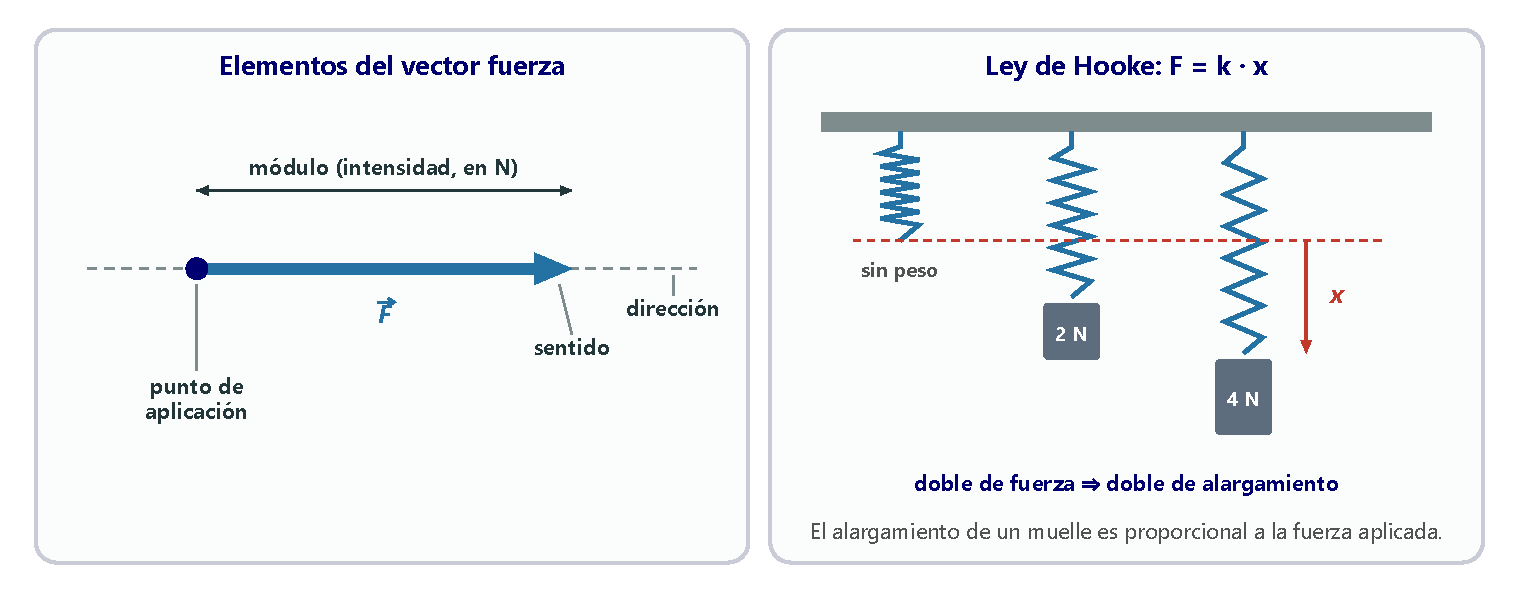
\includegraphics[width=0.85\textwidth]{images/UD10/vector_fuerza}
    \caption{Elementos de una fuerza y ley de Hooke: el alargamiento de un muelle es proporcional a la fuerza que lo estira.}
    \label{fig:ud10-vector}
\end{figure}

\subsection{Medida de las fuerzas}

Algunos materiales se deforman de manera proporcional a la fuerza que se les aplica, y esto permite medir fuerzas.

\begin{definition}[Dinamómetro]
    Es el instrumento que mide fuerzas. Consta de un muelle y una escala graduada, y se basa en la \textbf{ley de Hooke}:
    \[ F = k\,(L - L_0) = k\,\Delta L \]
    donde \(L_0\) es la longitud natural del muelle y \(L\) su longitud cuando actúa la fuerza.
\end{definition}

\begin{example}
    \textbf{Calibrar un muelle.} Un muelle mide \qty{15}{\cm} sin carga y \qty{18}{\cm} cuando se cuelga de él una pesa de
    \qty{6}{\newton}. a) ¿Cuál es su constante elástica? b) ¿Qué fuerza lo estira hasta \qty{22}{\cm}?

    \textbf{Solución.} a) \(k = \dfrac{F}{\Delta L} = \dfrac{6}{\num{0.03}} = \qty{200}{\newton\per\m}\).
    b) \(F = 200 \cdot \num{0.07} = \qty{14}{\newton}\).
\end{example}

\subsection{Clasificación de las fuerzas}

Las fuerzas nunca actúan aisladas: siempre son el resultado de una \textbf{interacción} entre, al menos, dos cuerpos. Podemos
clasificarlas de dos maneras.

\paragraph{Según la distancia entre los cuerpos.}
\begin{itemize}
    \item \textbf{Fuerzas de contacto}: necesitan que los cuerpos se toquen, como el empuje de una mano, la tensión de una cuerda o el
    rozamiento.
    \item \textbf{Fuerzas a distancia}: actúan sin contacto, como el peso o la atracción de un imán.
\end{itemize}

\paragraph{Interacciones fundamentales.} Todas las fuerzas de la naturaleza se deben, en último término, a cuatro tipos de
interacción entre partículas (tabla~\ref{tab:ud10-interacciones}). Las fuerzas de contacto, por ejemplo, son de origen
electromagnético: se deben a la repulsión entre los electrones de las superficies que se tocan.

\begin{table}[H]
    \centering
    \caption{Las cuatro interacciones fundamentales}
    \vspace{-5pt}
    \begin{tabular}{@{}lL{3.2cm}L{6.4cm}@{}}
        \toprule
        \textbf{Interacción} & \textbf{Alcance y carácter} & \textbf{Qué explica} \\
        \midrule
        Nuclear fuerte & Muy corto; atractiva; la más intensa & Mantiene unidos los quarks de protones y neutrones y estas
        partículas en el núcleo \\[3pt]
        Nuclear débil & Muy corto & Algunas desintegraciones radiactivas (como la desintegración beta) \\[3pt]
        Electromagnética & Largo; atractiva o repulsiva & Las propiedades de átomos y moléculas, la electricidad, el magnetismo, la
        luz y las fuerzas de contacto \\[3pt]
        Gravitatoria & Largo; siempre atractiva; la más débil & El peso, las mareas, el movimiento de los astros y la estructura del
        universo \\
        \bottomrule
    \end{tabular}
    \label{tab:ud10-interacciones}
\end{table}

\begin{remark}
    La física actual describe las interacciones mediante \textbf{campos}. Por ejemplo, en la teoría de la relatividad general de
    Einstein la gravedad no es una fuerza, sino una deformación del espacio-tiempo causada por la masa.
\end{remark}

\begin{exercise}
    Indica qué interacción fundamental actúa en cada caso: a) en una central nuclear se rompen núcleos de uranio; b) un imán atrae
    un clip; c) en un reactor experimental de fusión se unen núcleos de hidrógeno para formar helio; d) la Luna gira alrededor de la
    Tierra; e) un carbono-14 se transforma en nitrógeno-14 emitiendo un electrón.
    \begin{solu}
        a) \textcolor{red}{Nuclear fuerte} (y electromagnética, que separa los fragmentos). b) \textcolor{red}{Electromagnética}.
        c) \textcolor{red}{Nuclear fuerte} (y débil en algunas etapas). d) \textcolor{red}{Gravitatoria}. e) \textcolor{red}{Nuclear
        débil} (desintegración beta).
    \end{solu}
\end{exercise}

\begin{exercise}
    Clasifica estas fuerzas en fuerzas de contacto o a distancia: a) una grúa levanta un palé con un cable; b) un imán sujeta una
    nota en la nevera; c) un portero despeja el balón con los puños; d) el Sol atrae a Marte.
    \begin{solu}
        \textcolor{red}{De contacto: a y c. A distancia: b y d} (en b, también hay fuerzas de contacto entre la nota y la nevera).
    \end{solu}
\end{exercise}

%========================================================================================
\section{Componer y descomponer fuerzas}\label{sec:ud10-componer}
%========================================================================================

\textbf{Componer} fuerzas es sustituirlas por una sola que produzca el mismo efecto; \textbf{descomponer} una fuerza es sustituirla
por otras (sus componentes) cuya acción conjunta equivalga a ella. Ambos procedimientos son imprescindibles para resolver problemas
de equilibrio y de dinámica.

\subsection{Descomposición de una fuerza: componentes}

En el plano, cualquier fuerza \(\vec{F}\) que forme un ángulo \(\varphi\) con la parte positiva del eje \(X\) se puede escribir como la
suma de una fuerza paralela al eje \(X\) y otra paralela al eje \(Y\) (figura~\ref{fig:ud10-componentes}):
\[ \vec{F} = F_x\,\ivec + F_y\,\jvec = F\cos\varphi\;\ivec + F\sen\varphi\;\jvec \]

\begin{figure}[H]
    \centering
    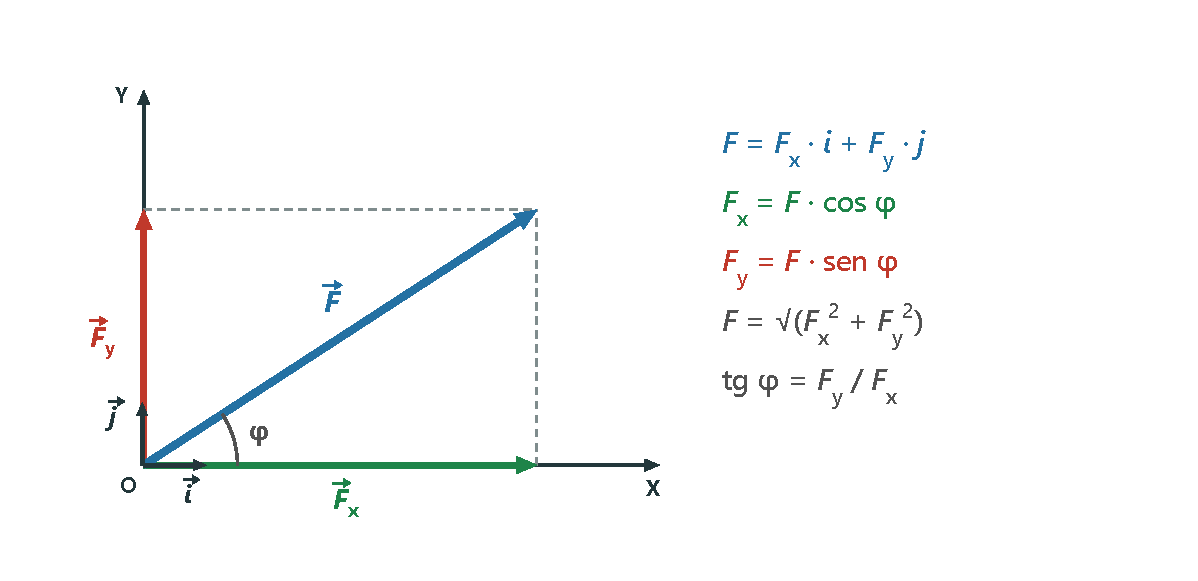
\includegraphics[width=0.75\textwidth]{images/UD10/descomposicion_fuerza}
    \caption{Componentes cartesianas de una fuerza. Conocidas las componentes, el módulo se obtiene con el teorema de Pitágoras y
    la dirección con la tangente.}
    \label{fig:ud10-componentes}
\end{figure}

\begin{example}
    \textbf{Tirar de un trineo.} Una persona tira de un trineo con una cuerda que forma \(30^\circ\) con el suelo, con una fuerza de
    \qty{500}{\newton}. Calcula las componentes horizontal y vertical de la fuerza y escríbela en forma vectorial.

    \textbf{Solución.} \(F_x = 500\cos 30^\circ = \qty{433}{\newton}\) (la que hace avanzar el trineo);
    \(F_y = 500\sen 30^\circ = \qty{250}{\newton}\) (tiende a levantarlo). En forma vectorial: \(\vec{F} = (433\,\ivec + 250\,\jvec)\)~N.
\end{example}

\subsection{Composición de fuerzas: fuerza resultante}

\begin{definition}[Fuerza resultante o neta]
    Es la suma vectorial de todas las fuerzas que actúan sobre un cuerpo, y produce por sí sola el mismo efecto que todas ellas:
    \[ \vec{F}_{\text{neta}} = \sum_{i=1}^{n} \vec{F}_i = \vec{F}_1 + \vec{F}_2 + \dots + \vec{F}_n
    = \Bigl(\sum F_{ix}\Bigr)\,\ivec + \Bigl(\sum F_{iy}\Bigr)\,\jvec \]
\end{definition}

Para fuerzas concurrentes, la resultante se calcula con la fórmula anterior (sumando componentes) o gráficamente. Hay casos
sencillos que conviene recordar (figura~\ref{fig:ud10-composicion}):

\begin{itemize}
    \item \textbf{Misma dirección y sentido}: los módulos se suman, \(F_{\text{neta}} = F_1 + F_2\).
    \item \textbf{Misma dirección y sentidos opuestos}: los módulos se restan, \(F_{\text{neta}} = |F_1 - F_2|\), y la resultante
    tiene el sentido de la mayor.
    \item \textbf{Fuerzas perpendiculares}: por el teorema de Pitágoras, \(F_{\text{neta}} = \sqrt{F_1^2 + F_2^2}\).
    \item \textbf{Cualquier ángulo \(\alpha\) entre ellas} (regla del paralelogramo):
    \(F_{\text{neta}} = \sqrt{F_1^2 + F_2^2 + 2F_1F_2\cos\alpha}\).
\end{itemize}

\begin{figure}[H]
    \centering
    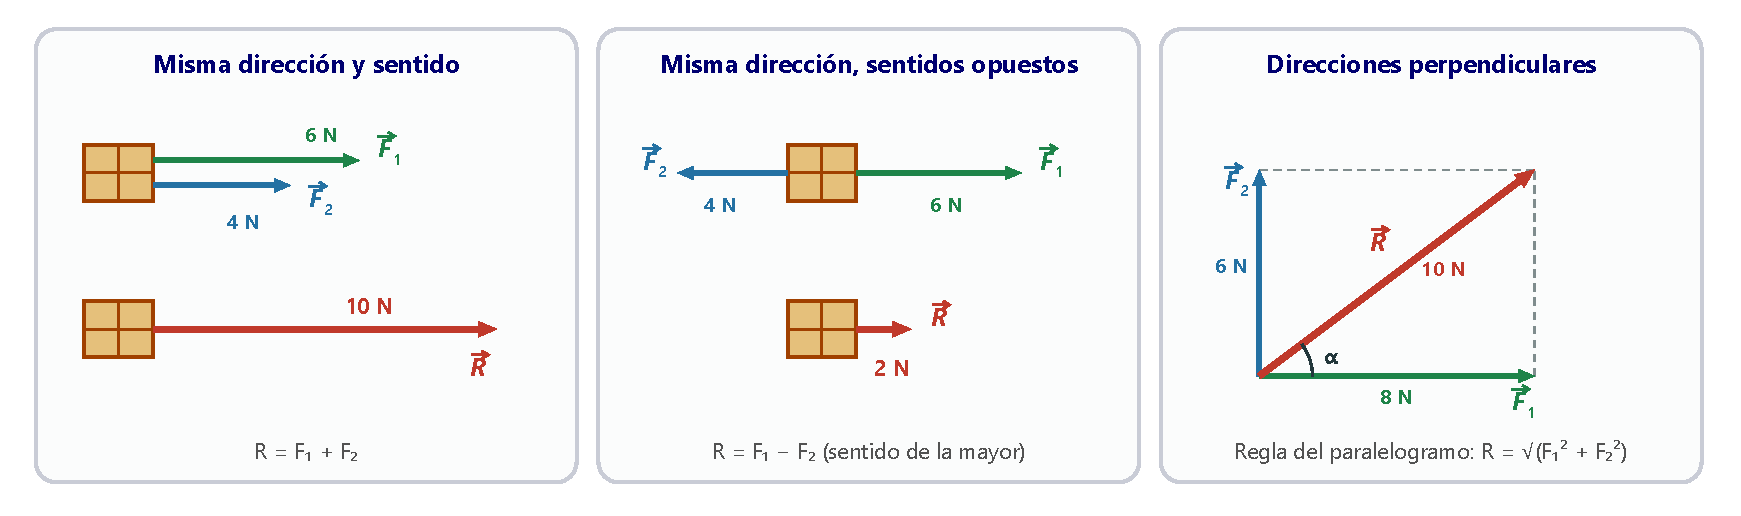
\includegraphics[width=\textwidth]{images/UD10/composicion_fuerzas}
    \caption{Resultante de dos fuerzas concurrentes en los tres casos más sencillos.}
    \label{fig:ud10-composicion}
\end{figure}

\begin{example}
    \textbf{Dos remolcadores.} Un buque mercante es arrastrado en el puerto por dos remolcadores que tiran en la misma dirección y
    sentido con fuerzas de \qty{2.6e5}{\newton} y \qty{3.4e5}{\newton}. a) ¿Qué fuerza total actúa sobre el buque? b) Si el buque
    pone en marcha sus motores en sentido contrario, con una fuerza de \qty{4.5e5}{\newton}, ¿cuál es la resultante?

    \textbf{Solución.} a) Misma dirección y sentido: \(F = \num{2.6e5} + \num{3.4e5} = \qty{6.0e5}{\newton}\).
    b) Sentidos opuestos: \(F' = \num{6.0e5} - \num{4.5e5} = \qty{1.5e5}{\newton}\), en el sentido de los remolcadores.
\end{example}

\begin{example}
    \textbf{Dos fuerzas que forman 60°.} Sobre un cuerpo actúan dos fuerzas de \qty{40}{\newton} y \qty{30}{\newton} que forman
    \(60^\circ\). Calcula el módulo de la resultante y el ángulo que forma con la fuerza mayor.

    \textbf{Solución.} Tomamos el eje \(X\) en la dirección de la fuerza de \qty{40}{\newton}:
    \(\vec{F}_1 = 40\,\ivec\) y \(\vec{F}_2 = 30\cos 60^\circ\,\ivec + 30\sen 60^\circ\,\jvec = 15\,\ivec + \num{25.98}\,\jvec\). Sumando:
    \(\vec{F} = 55\,\ivec + \num{25.98}\,\jvec\)~N.
    \[ F = \sqrt{55^2 + \num{25.98}^2} = \qty{60.8}{\newton} \qquad \tg\varphi = \frac{\num{25.98}}{55} \Rightarrow \varphi = \num{25.3}^\circ \]
    Con la regla del paralelogramo: \(F = \sqrt{1600 + 900 + 2 \cdot 40 \cdot 30 \cdot \cos 60^\circ} = \sqrt{3700} = \qty{60.8}{\newton}\).
\end{example}

\begin{exercise}
    Dibuja y calcula la resultante de tres fuerzas concurrentes de 16, 9 y \qty{25}{\newton}. Las fuerzas de 9 y \qty{25}{\newton}
    tienen la misma dirección y sentidos opuestos, y la de \qty{16}{\newton} es perpendicular a ellas.
    \begin{solu}
        \textcolor{blue}{En la dirección de las dos primeras: \(25 - 9 = \qty{16}{\newton}\); perpendicular: \qty{16}{\newton}.}
        \(F = \sqrt{16^2 + 16^2} = \textcolor{red}{\qty{22.6}{\newton}}\), formando \(45^\circ\) con cada dirección.
    \end{solu}
\end{exercise}

\begin{exercise}
    Calcula la resultante de \(\vec{F}_1 = (3\,\ivec + 5\,\jvec)\)~N, \(\vec{F}_2 = (-7\,\ivec + 2\,\jvec)\)~N y
    \(\vec{F}_3 = (6\,\ivec - 4\,\jvec)\)~N, su módulo y el ángulo que forma con el eje \(X\).
    \begin{solu}
        \(\vec{F} = (3 - 7 + 6)\,\ivec + (5 + 2 - 4)\,\jvec = \textcolor{red}{(2\,\ivec + 3\,\jvec)~\text{N}}\);
        \(F = \sqrt{13} = \textcolor{red}{\qty{3.61}{\newton}}\); \(\tg\varphi = \num{1.5} \Rightarrow \textcolor{red}{\varphi = \num{56.3}^\circ}\).
    \end{solu}
\end{exercise}

%========================================================================================
\section{El equilibrio}\label{sec:ud10-equilibrio}
%========================================================================================

En la vida diaria encontramos muchas situaciones de equilibrio: una persona haciendo una postura de yoga, un puente, un tren que
avanza por una vía recta a velocidad constante o una noria que gira siempre al mismo ritmo.

\subsection{Equilibrio de un cuerpo puntual}

\begin{definition}[Equilibrio de un cuerpo puntual]
    Un cuerpo puntual está en \textbf{equilibrio} si la resultante de todas las fuerzas que actúan sobre él es nula:
    \[ \sum \vec{F}_i = \vec{0} \quad\Longleftrightarrow\quad \sum F_{ix} = 0 \quad \text{y} \quad \sum F_{iy} = 0 \]
\end{definition}

\paragraph{Reposo y equilibrio.} Son conceptos distintos que a menudo se confunden:
\begin{itemize}
    \item Un cuerpo está en \textbf{reposo} si su velocidad es nula.
    \item Un cuerpo está en \textbf{equilibrio} si la fuerza neta sobre él es nula, es decir, si no tiene aceleración.
\end{itemize}
En un MRU hay \textbf{equilibrio sin reposo}: el cuerpo se mueve, pero sin aceleración. Y un objeto lanzado verticalmente hacia arriba
está en \textbf{reposo} instantáneo en el punto más alto, pero \textbf{no en equilibrio}, porque sobre él sigue actuando su peso.

\begin{figure}[H]
    \centering
    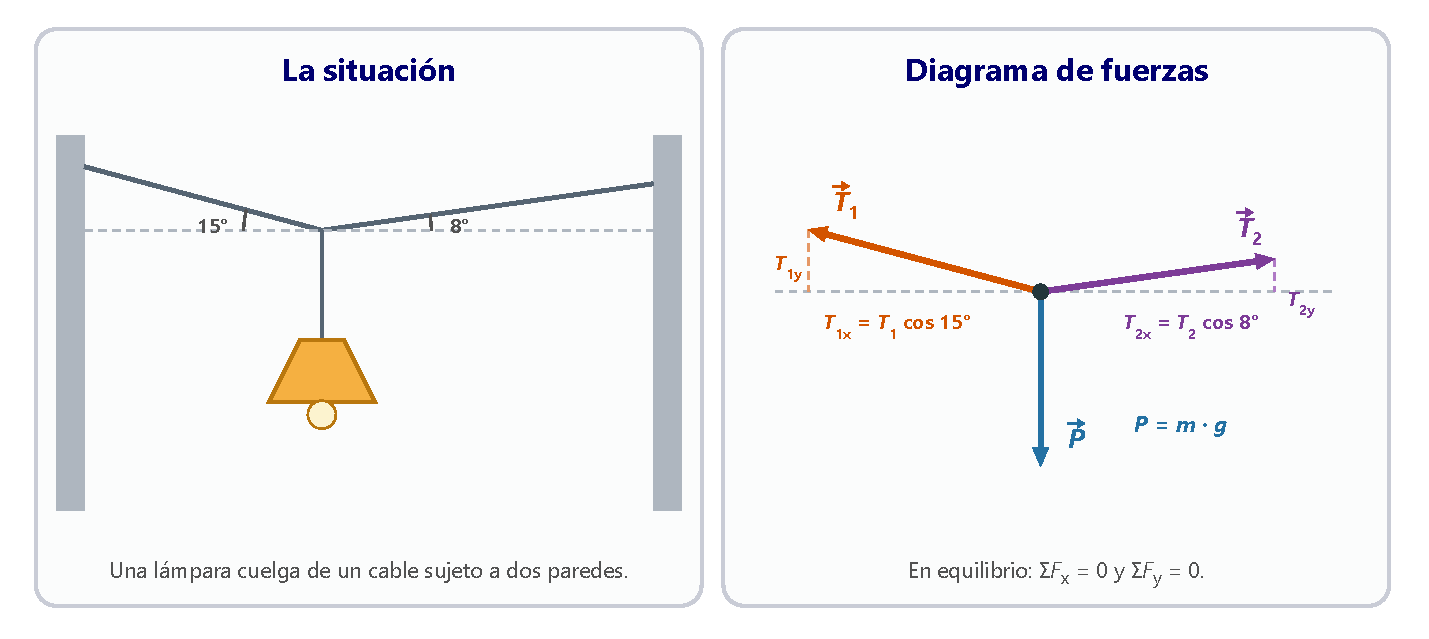
\includegraphics[width=0.95\textwidth]{images/UD10/equilibrio_cuerda}
    \caption{Un cuerpo colgado de un cable: el punto de unión está en equilibrio bajo la acción de las dos tensiones y el peso.}
    \label{fig:ud10-cuerda}
\end{figure}

\begin{example}
    \textbf{Una lámpara colgada de un cable.} Una lámpara de \qty{2.5}{\kg} cuelga del punto de un cable en el que este forma
    ángulos de \(15^\circ\) y \(8^\circ\) con la horizontal (figura~\ref{fig:ud10-cuerda}). Calcula la tensión de cada tramo del cable.

    \textbf{Solución.} Sobre el punto de unión actúan el peso, \(P = \num{2.5} \cdot \num{9.8} = \qty{24.5}{\newton}\), y las tensiones
    \(T_1\) (a la izquierda) y \(T_2\) (a la derecha). Aplicamos las condiciones de equilibrio:

    Eje \(X\): \(T_2\cos 8^\circ = T_1\cos 15^\circ \Rightarrow T_2 = \dfrac{\cos 15^\circ}{\cos 8^\circ}\,T_1 = \num{0.9754}\,T_1\)

    Eje \(Y\): \(T_1\sen 15^\circ + T_2\sen 8^\circ = P \Rightarrow T_1\,(\num{0.2588} + \num{0.9754} \cdot \num{0.1392}) = \num{24.5}\)
    \[ T_1 = \frac{\num{24.5}}{\num{0.3946}} = \qty{62.1}{\newton} \qquad T_2 = \num{0.9754} \cdot \num{62.1} = \qty{60.6}{\newton} \]
    Las tensiones son mucho mayores que el peso: cuanto más horizontal está un cable, más tenso tiene que estar para sujetar la carga.
\end{example}

\begin{exercise}
    Un contenedor de \qty{600}{\kg} cuelga de dos cables iguales que forman \(20^\circ\) con la horizontal. Calcula la tensión de
    cada cable.
    \begin{solu}
        \textcolor{blue}{Por simetría, las dos tensiones son iguales: \(2T\sen 20^\circ = m\,g\).}
        \(T = \dfrac{600 \cdot \num{9.8}}{2\sen 20^\circ} = \textcolor{red}{\qty{8.60e3}{\newton}}\).
    \end{solu}
\end{exercise}

\subsection{Momento de una fuerza}

Hasta ahora hemos supuesto que las fuerzas desplazan los cuerpos (traslación), pero también pueden hacerlos \textbf{girar}. Si la
línea de acción de una fuerza no pasa por el centro de masas de un cuerpo o por su eje de giro, la fuerza produce una
\textbf{rotación}. La magnitud que mide esta capacidad es el \textbf{momento de la fuerza}.

\begin{definition}[Momento de una fuerza]
    El momento de una fuerza \(\vec{F}\) respecto a un punto O es el vector
    \[ \vec{M} = \vec{r} \times \vec{F} \]
    donde \(\vec{r}\) es el vector de posición del punto de aplicación de la fuerza respecto a O. Mide la capacidad de la fuerza para
    cambiar la velocidad de giro del cuerpo.
\end{definition}

Sus características son (figura~\ref{fig:ud10-momento}):
\begin{itemize}
    \item \textbf{Módulo}: \(M = r\,F\sen\varphi\), donde \(\varphi\) es el ángulo entre \(\vec{r}\) y \(\vec{F}\). Se mide en
    \unit{\newton\metre}.
    \item \textbf{Dirección}: perpendicular al plano formado por \(\vec{r}\) y \(\vec{F}\) (la del eje de giro).
    \item \textbf{Sentido}: por convenio, positivo si el giro es antihorario y negativo si es horario.
\end{itemize}
Si la línea de acción de la fuerza pasa por O (\(\varphi = 0^\circ\) o \(180^\circ\)), el momento es nulo: empujar una puerta hacia
las bisagras no la hace girar.

\begin{figure}[H]
    \centering
    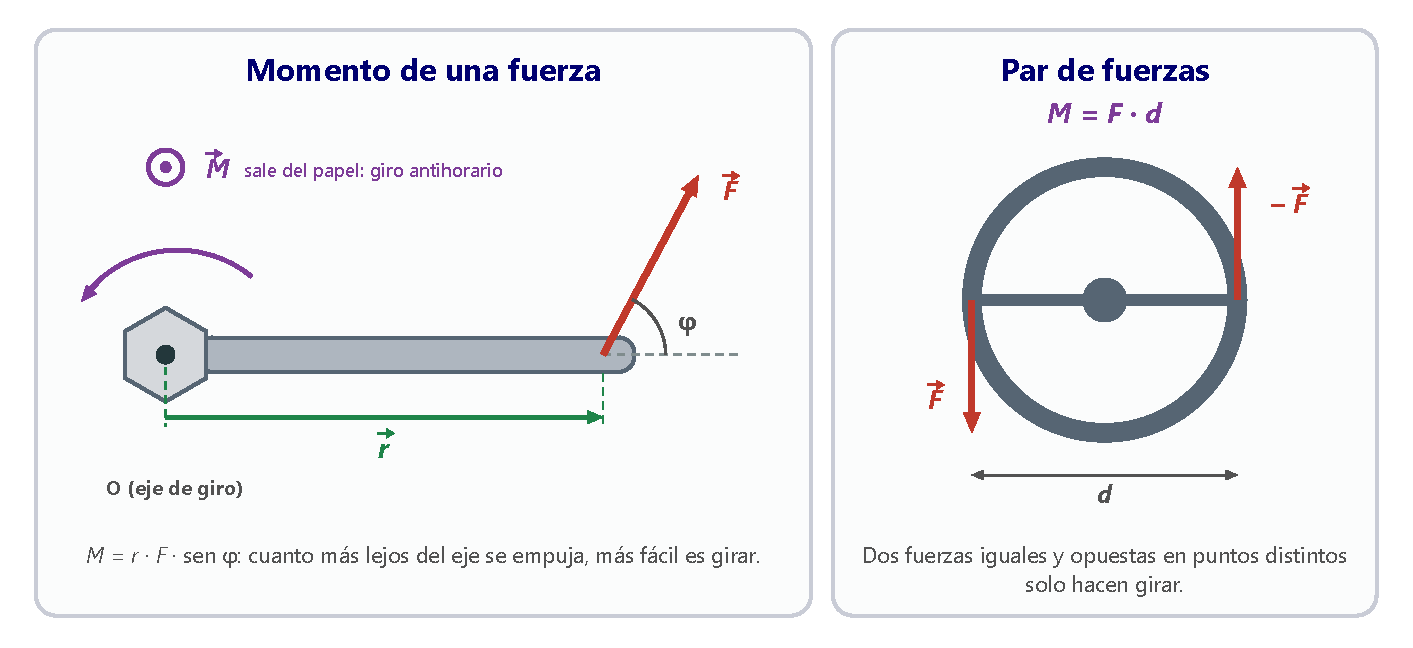
\includegraphics[width=0.95\textwidth]{images/UD10/momento_fuerza}
    \caption{Momento de una fuerza aplicada a una llave inglesa y par de fuerzas sobre un volante.}
    \label{fig:ud10-momento}
\end{figure}

\begin{definition}[Par de fuerzas]
    Un \textbf{par de fuerzas} son dos fuerzas paralelas, de igual módulo y sentidos contrarios, aplicadas en puntos distintos. Su
    resultante es nula, así que no trasladan el cuerpo, pero lo hacen girar con un momento \(M = F\,d\), donde \(d\) es la distancia
    entre sus líneas de acción. Es lo que hacemos al girar un volante o un grifo.
\end{definition}

\begin{example}
    \textbf{Cambiar una rueda.} Para aflojar una tuerca se usa una llave de \qty{30}{\cm} y se aplica en su extremo una fuerza de
    \qty{80}{\newton}. a) Calcula el momento si la fuerza es perpendicular a la llave. b) ¿Y si forma \(60^\circ\) con ella?

    \textbf{Solución.} a) \(M = r\,F\sen 90^\circ = \num{0.30} \cdot 80 \cdot 1 = \qty{24}{\newton\metre}\).
    b) \(M = \num{0.30} \cdot 80 \cdot \sen 60^\circ = \qty{20.8}{\newton\metre}\). El momento es máximo cuando la fuerza es
    perpendicular a la llave.
\end{example}

\subsection{Equilibrio de un cuerpo extenso}

Una fuerza neta hace que un cuerpo empiece a trasladarse o cambie su movimiento de traslación; un momento neto hace que empiece a
girar o cambie su rotación.

\begin{definition}[Condiciones de equilibrio de un sólido]
    Un cuerpo extenso está en equilibrio si son nulas la resultante de las fuerzas y la resultante de los momentos respecto a
    cualquier punto:
    \[ \sum \vec{F}_i = \vec{0} \qquad \sum \vec{M}_i = \vec{0} \]
\end{definition}

\begin{remark}
    Hay tres tipos de equilibrio: \textbf{estático} (el cuerpo está en reposo, como una persona en una postura de yoga),
    \textbf{dinámico} (se traslada con velocidad constante, como un tren en una recta) y \textbf{rotacional} (gira con velocidad angular
    constante, como una rueda de molino).
\end{remark}

\begin{example}
    \textbf{Transportar un saco.} Dos personas llevan un saco de \qty{60}{\kg} colgado de una barra de peso despreciable. Una está a
    \qty{0.9}{\m} del saco y la otra a \qty{1.5}{\m}. ¿Qué fuerza hace cada una?

    \textbf{Solución.} El peso del saco es \(P = 60 \cdot \num{9.8} = \qty{588}{\newton}\). Condiciones de equilibrio:
    \[ \sum F = 0:\; F_1 + F_2 = P \qquad \sum M_{\text{saco}} = 0:\; F_1 \cdot \num{0.9} = F_2 \cdot \num{1.5} \]
    Tomando momentos respecto al punto del que cuelga el saco (así el peso no da momento):
    \(F_1 = \dfrac{\num{1.5}}{\num{0.9}}\,F_2\). Sustituyendo: \(F_2\left(1 + \dfrac{\num{1.5}}{\num{0.9}}\right) = 588 \Rightarrow
    F_2 = \qty{220.5}{\newton}\) y \(F_1 = \qty{367.5}{\newton}\). Hace más fuerza la persona que está \textbf{más cerca} del saco.
\end{example}

\begin{exercise}
    Dos fuerzas paralelas de \qty{10}{\newton} y \qty{40}{\newton}, ambas hacia abajo, actúan en los extremos de una barra de
    \qty{2.5}{\m} de peso despreciable. ¿Dónde hay que colocar el punto de apoyo para que la barra esté en equilibrio? ¿Qué fuerza
    hace el apoyo?
    \begin{solu}
        \textcolor{blue}{Momentos respecto al apoyo, a una distancia \(x\) de la fuerza de \qty{10}{\newton}: \(10\,x = 40\,(\num{2.5} - x)\).}
        \(x = \textcolor{red}{\qty{2}{\m}}\) de la fuerza de \qty{10}{\newton} (a \qty{0.5}{\m} de la de \qty{40}{\newton}). El
        apoyo hace \(\textcolor{red}{\qty{50}{\newton}}\) hacia arriba.
    \end{solu}
\end{exercise}

\begin{exercise}
    El tablero de una mesa mide \qty{2.4}{\m} y pesa \qty{60}{\newton}. Se apoya en dos caballetes: uno en un extremo y otro a
    \qty{0.6}{\m} del otro extremo. Calcula la fuerza que hace cada caballete.
    \begin{solu}
        \textcolor{blue}{El peso actúa en el centro del tablero, a \qty{1.2}{\m} del extremo apoyado.}
        \textcolor{blue}{Los caballetes distan \qty{1.8}{\m}.} Tomamos momentos respecto al caballete del extremo:
        \[ F_B \cdot \num{1.8} = 60 \cdot \num{1.2} \]
        \(\textcolor{red}{F_B = \qty{40}{\newton}}\) y \(\textcolor{red}{F_A = 60 - 40 = \qty{20}{\newton}}\).
    \end{solu}
\end{exercise}

\begin{exercise}
    Para abrir una puerta de \qty{85}{\cm} de anchura hace falta un momento de \qty{1.5}{\newton\metre}. Si empujamos
    perpendicularmente junto al pomo con una fuerza de \qty{2}{\newton}, ¿se abrirá? ¿Y si empujamos con la misma fuerza a
    \qty{40}{\cm} de las bisagras?
    \begin{solu}
        Junto al pomo: \(M = \num{0.85} \cdot 2 = \qty{1.7}{\newton\metre}\), \textcolor{red}{sí se abre}. A \qty{40}{\cm}:
        \(M = \num{0.40} \cdot 2 = \qty{0.8}{\newton\metre}\), \textcolor{red}{no se abre}.
    \end{solu}
\end{exercise}

%========================================================================================
\section{Las leyes de Newton}\label{sec:ud10-newton}
%========================================================================================

La \textbf{dinámica} es la parte de la física que estudia el movimiento de los cuerpos atendiendo a sus causas, las fuerzas. Toda la
dinámica clásica se basa en las tres \textbf{leyes de Newton}, que relacionan las fuerzas que actúan sobre un cuerpo con su movimiento.
Newton las publicó en 1687 en su obra \textit{Philosophiae Naturalis Principia Mathematica}.

\subsection{Primera ley de Newton: principio de inercia}

Cuando vamos en moto y arrancamos, notamos que nos vamos hacia atrás; si frenamos de golpe, nos vamos hacia delante. En ambos casos
el cuerpo tiende a \textbf{mantener su estado}: en reposo o moviéndose en línea recta a velocidad constante. Solo cuando el asiento
o el manillar nos empujan pasamos a movernos con la moto.

\begin{definition}[Inercia]
    Es la tendencia de un cuerpo a mantener su estado de reposo o de movimiento rectilíneo uniforme. Es una propiedad de toda la
    materia y está ligada a la masa: cuanto mayor es la masa, mayor es la inercia.
\end{definition}

\begin{definition}[Primera ley de Newton o principio de inercia]
    Si sobre un cuerpo no actúa ninguna fuerza, o la resultante de las que actúan es nula, el cuerpo permanece en reposo o se mueve
    con movimiento rectilíneo uniforme:
    \[ \sum \vec{F}_i = \vec{0} \quad\Longrightarrow\quad \vec{v} = \text{constante} \]
\end{definition}

Si la velocidad constante es \(\vec{0}\), el cuerpo está en reposo; si es distinta de cero, el cuerpo describe un MRU.

\paragraph{Sistemas de referencia inerciales.} Un \textbf{sistema de referencia inercial} es aquel en el que se cumple el principio
de inercia. Todos los sistemas que se mueven con MRU respecto a uno inercial son también inerciales.

\begin{definition}[Principio de relatividad de Galileo]
    Las leyes de la mecánica son las mismas en todos los sistemas de referencia inerciales.
\end{definition}

Por eso, con experimentos mecánicos es imposible distinguir si un sistema inercial está en reposo o se mueve con MRU: \textbf{no se
puede medir el movimiento absoluto}. El tiempo, la masa y las fuerzas tienen el mismo valor en todos los sistemas inerciales: son
\textbf{invariantes de Galileo}. Einstein amplió este principio a todas las leyes de la física en su teoría de la relatividad
(1905), en la que longitudes y tiempos sí dependen del sistema de referencia cuando las velocidades se acercan a la de la luz.

\begin{remark}
    En rigor, la Tierra \textbf{no} es un sistema inercial, porque gira sobre sí misma y alrededor del Sol. Pero sus aceleraciones
    son tan pequeñas que, para la mayoría de los movimientos cotidianos, podemos tratarla como si lo fuera.
\end{remark}

\begin{example}
    \textbf{En un avión.} Explica qué le ocurre a una persona sentada en un avión cuando: a) el avión gira hacia la izquierda;
    b) despega; c) aterriza y frena; d) desciende bruscamente.

    \textbf{Solución.} Por el principio de inercia, la persona tiende a seguir moviéndose como lo hacía: a) sigue en línea recta,
    así que respecto al avión se desplaza hacia la \textbf{derecha}; b) tiende a quedarse atrás y se siente \textbf{empujada contra el
    respaldo}; c) sigue moviéndose y se va \textbf{hacia delante}; d) tiende a seguir a la misma altura, así que se siente
    \textbf{levantada del asiento}.
\end{example}

\begin{exercise}
    Cuando viajamos con una mascota en el coche, la ley obliga a llevarla sujeta y separada del conductor. Explica por qué con la
    primera ley de Newton. ¿Qué ocurriría con la mascota y con los pasajeros sin cinturón en un frenazo brusco?
    \begin{solu}
        \textcolor{red}{En un frenazo, por inercia, todo lo que no está sujeto sigue moviéndose hacia delante a la velocidad que
        llevaba el coche} y choca contra los asientos, el parabrisas o los pasajeros. Los cinturones y los arneses ejercen la fuerza
        necesaria para frenarlos junto con el coche.
    \end{solu}
\end{exercise}

\begin{exercise}
    En un truco de magia se tira bruscamente de un mantel y los platos y vasos que hay encima apenas se mueven. Explica el fenómeno
    y propón otros ejemplos basados en el mismo principio.
    \begin{solu}
        Es el \textcolor{red}{principio de inercia}: si el tirón es muy rápido, la fuerza de rozamiento actúa durante muy poco tiempo
        y apenas cambia el estado de reposo de los platos. Otros ejemplos: la moneda sobre una cartulina que se retira de un golpe
        (práctica~\ref{sec:ud10-practicas}), quitar una pieza de la base de una torre de bloques de un golpe seco, sacudir una
        alfombra para quitarle el polvo.
    \end{solu}
\end{exercise}

\subsection{Segunda ley de Newton: principio fundamental de la dinámica}

La primera ley describe qué ocurre cuando la fuerza neta es nula. La segunda explica qué ocurre cuando no lo es: la fuerza neta es
la responsable de los \textbf{cambios} de velocidad.

\begin{definition}[Segunda ley de Newton o principio fundamental de la dinámica]
    La fuerza neta que actúa sobre un cuerpo le produce una aceleración de la misma dirección y sentido, directamente proporcional a
    la fuerza e inversamente proporcional a la masa del cuerpo:
    \[ \sum \vec{F}_i = \vec{F}_{\text{neta}} = m\,\vec{a} \]
\end{definition}

Si se aplican a un mismo cuerpo distintas fuerzas, el cociente entre cada fuerza y la aceleración que produce es siempre el mismo, la
masa inercial: \(\dfrac{F_1}{a_1} = \dfrac{F_2}{a_2} = \dots = m\). Cuanto mayor es la masa de un cuerpo, mayor es su inercia y más
fuerza hace falta para cambiar su movimiento. De esta ley sale la definición del newton: \textbf{\qty{1}{\newton} es la fuerza que
comunica a una masa de \qty{1}{\kg} una aceleración de \qty{1}{\m\per\s\squared}}.

\begin{remark}
    La fuerza neta y la aceleración tienen siempre la misma dirección y sentido, pero no necesariamente la velocidad. Conocidas la
    velocidad inicial y la aceleración, las ecuaciones de la cinemática de la unidad anterior nos dicen cómo evoluciona el movimiento.
\end{remark}

\paragraph{Cómo resolver un problema de dinámica.}
\begin{enumerate}[label=\numberballgreen]
    \item Dibuja \textbf{todas las fuerzas} que actúan sobre el cuerpo (y solo esas).
    \item Elige unos ejes: uno en la dirección del movimiento y otro perpendicular.
    \item Descompón las fuerzas que no estén sobre los ejes.
    \item Aplica \(\sum F_x = m\,a\) en la dirección del movimiento y \(\sum F_y = 0\) en la perpendicular.
\end{enumerate}

\begin{example}
    \textbf{Una grúa remolca un coche.} Una grúa arrastra un coche averiado de \qty{1100}{\kg} con un cable que forma \(20^\circ\)
    con la horizontal y ejerce una fuerza de \qty{12000}{\newton}. La fuerza de rozamiento es de \qty{3500}{\newton}. Calcula: a) la
    aceleración del coche; b) la distancia que recorre en \qty{5}{\s} si parte del reposo.

    \textbf{Solución.} a) En el eje del movimiento actúan la componente horizontal de la fuerza del cable y el rozamiento:
    \[ F_x = 12000\cos 20^\circ = \qty{11276}{\newton} \qquad F_x - F_r = m\,a \Rightarrow a = \frac{11276 - 3500}{1100} = \qty{7.07}{\m\per\s\squared} \]
    (En el eje vertical no hay aceleración: el peso queda compensado por la normal y la componente vertical de la fuerza del cable.)

    b) Con la ecuación del MRUA: \(x = \dfrac{1}{2}\,a\,t^2 = \dfrac{1}{2} \cdot \num{7.07} \cdot 5^2 = \qty{88.4}{\m}\).
\end{example}

\paragraph{El plano inclinado.} Sobre un cuerpo apoyado en un plano inclinado un ángulo \(\alpha\) actúan su peso, la normal y, si
lo hay, el rozamiento. Conviene tomar un eje paralelo al plano y otro perpendicular, y descomponer el peso
(figura~\ref{fig:ud10-plano}):
\[ P_x = m\,g\sen\alpha \qquad P_y = m\,g\cos\alpha \]
La componente paralela, \(P_x\), hace bajar el cuerpo; la perpendicular, \(P_y\), la equilibra la normal.

\begin{figure}[H]
    \centering
    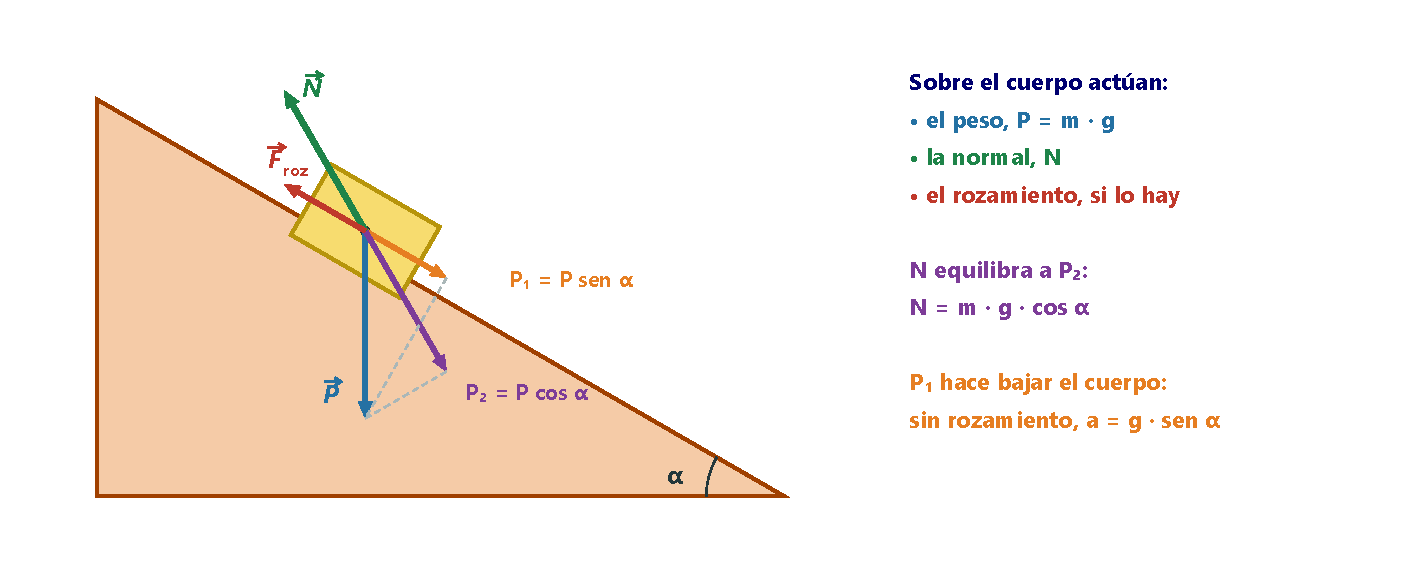
\includegraphics[width=0.85\textwidth]{images/UD10/plano_inclinado}
    \caption{Fuerzas sobre un cuerpo en un plano inclinado. Las componentes del peso se nombran aquí \(P_1\) (paralela) y \(P_2\)
    (perpendicular).}
    \label{fig:ud10-plano}
\end{figure}

\begin{example}
    \textbf{Una bola por una rampa.} Una bola de \qty{2}{\kg} baja por un plano inclinado \(25^\circ\) y sobre ella actúa una fuerza
    de rozamiento de \qty{2}{\newton}. Calcula: a) su aceleración; b) el tiempo que tarda en recorrer \qty{6}{\m} si parte del reposo.

    \textbf{Solución.} a) Peso: \(P = 2 \cdot \num{9.8} = \qty{19.6}{\newton}\); \(P_x = \num{19.6}\sen 25^\circ = \qty{8.28}{\newton}\);
    \(P_y = \num{19.6}\cos 25^\circ = \qty{17.8}{\newton} = N\).
    \[ P_x - F_r = m\,a \Rightarrow a = \frac{\num{8.28} - 2}{2} = \qty{3.14}{\m\per\s\squared} \]
    b) \(x = \dfrac{1}{2}\,a\,t^2 \Rightarrow t = \sqrt{\dfrac{2x}{a}} = \sqrt{\dfrac{2 \cdot 6}{\num{3.14}}} = \qty{1.95}{\s}\).
\end{example}

\begin{exercise}
    Una caja de \qty{90}{\kg}, en reposo sobre el suelo, es empujada horizontalmente con una fuerza de \qty{320}{\newton}. Si la
    fuerza de rozamiento es de \qty{230}{\newton}, ¿qué velocidad tendrá al cabo de \qty{4}{\s}?
    \begin{solu}
        \(a = \dfrac{320 - 230}{90} = \qty{1}{\m\per\s\squared}\); \(v = a\,t = \textcolor{red}{\qty{4}{\m\per\s}}\).
    \end{solu}
\end{exercise}

\begin{exercise}
    Sobre un sillón de \qty{70}{\kg} en reposo se aplica una fuerza horizontal de \qty{420}{\newton}. El rozamiento es de
    \qty{280}{\newton}. Calcula: a) la aceleración; b) la velocidad y la distancia recorrida en \qty{4}{\s}.
    \begin{solu}
        a) \(a = \dfrac{420 - 280}{70} = \textcolor{red}{\qty{2}{\m\per\s\squared}}\). b) \(v = 2 \cdot 4 = \textcolor{red}{\qty{8}{\m\per\s}}\);
        \(x = \frac{1}{2} \cdot 2 \cdot 4^2 = \textcolor{red}{\qty{16}{\m}}\).
    \end{solu}
\end{exercise}

\begin{exercise}
    Un técnico de sonido sube unos altavoces de \qty{70}{\kg} por una rampa inclinada \(15^\circ\). Si el rozamiento es de
    \qty{150}{\newton}, ¿qué fuerza mínima, paralela a la rampa, debe hacer?
    \begin{solu}
        \textcolor{blue}{La fuerza mínima es la que consigue que suban a velocidad constante (\(a = 0\)):}
        \(F = m\,g\sen 15^\circ + F_r = \num{177.5} + 150 = \textcolor{red}{\qty{328}{\newton}}\).
    \end{solu}
\end{exercise}

\begin{exercise}
    Sobre un cuerpo de \qty{8}{\kg} situado en un plano inclinado \(30^\circ\) se aplica una fuerza de \qty{12}{\newton} paralela
    al plano y hacia abajo. El rozamiento es de \qty{10}{\newton}. a) Calcula la aceleración. b) Si se retira la fuerza de
    \qty{12}{\newton}, ¿qué fuerza hay que aplicar hacia arriba para que el cuerpo baje con velocidad constante?
    \begin{solu}
        \(P_x = 8 \cdot \num{9.8} \cdot \sen 30^\circ = \qty{39.2}{\newton}\). a) \(a = \dfrac{12 + \num{39.2} - 10}{8} =
        \textcolor{red}{\qty{5.15}{\m\per\s\squared}}\). b) \(F + F_r = P_x \Rightarrow F = \num{39.2} - 10 =
        \textcolor{red}{\qty{29.2}{\newton}}\).
    \end{solu}
\end{exercise}

\subsection{Tercera ley de Newton: principio de acción y reacción}

Las dos primeras leyes se fijan en un solo cuerpo y en las fuerzas que actúan sobre él. La tercera nos recuerda que una fuerza es
siempre una \textbf{interacción} entre dos cuerpos: un cuerpo no puede, por sí solo, cambiar su estado de movimiento.

\begin{definition}[Tercera ley de Newton o principio de acción y reacción]
    Si un cuerpo A ejerce una fuerza sobre un cuerpo B, el cuerpo B ejerce sobre A una fuerza de igual módulo y dirección y de
    sentido contrario:
    \[ \vec{F}_{AB} = -\vec{F}_{BA} \]
    A estas dos fuerzas se las llama \textbf{acción} y \textbf{reacción}.
\end{definition}

Hay que tener en cuenta que:
\begin{itemize}
    \item Las fuerzas siempre aparecen \textbf{por pares}: a cada acción le corresponde una reacción.
    \item Acción y reacción son \textbf{simultáneas}: no hay una primera y otra después.
    \item Actúan sobre \textbf{cuerpos distintos}, por lo que \textbf{no se anulan} entre sí. Sus efectos pueden ser muy diferentes: el
    cuerpo de mayor masa adquiere menor aceleración.
\end{itemize}

\begin{figure}[H]
    \centering
    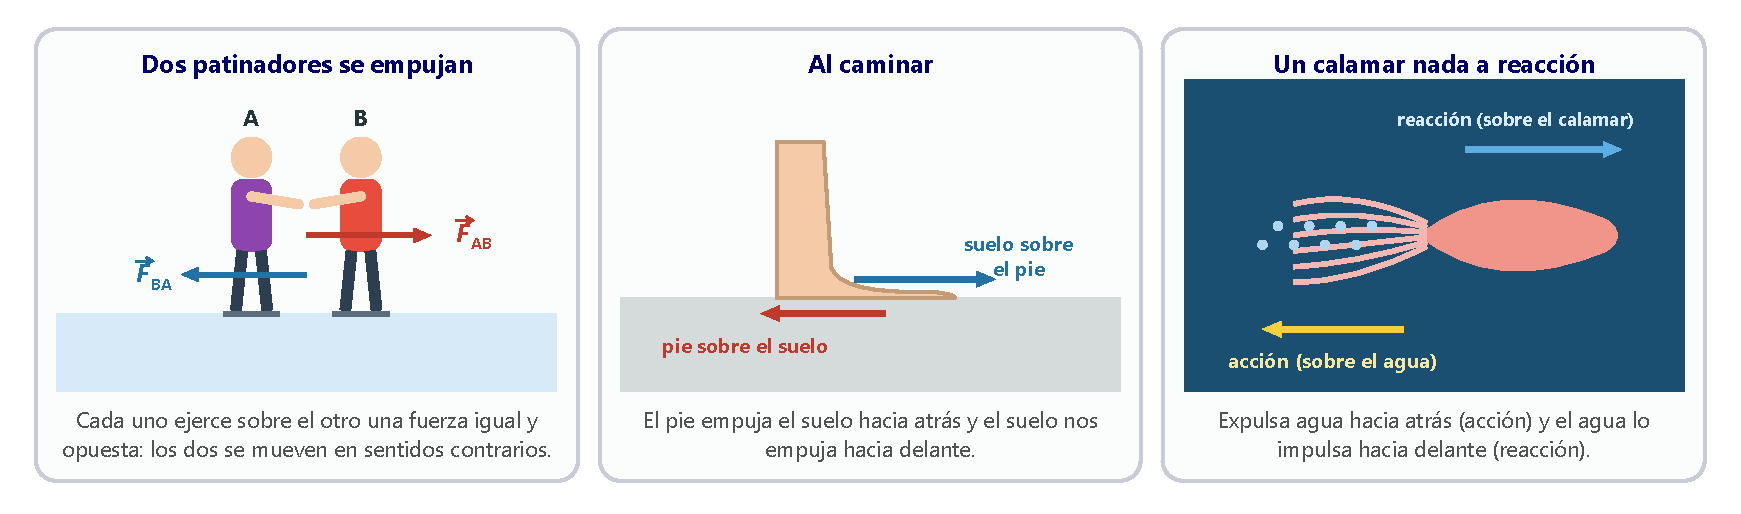
\includegraphics[width=\textwidth]{images/UD10/accion_reaccion}
    \caption{Ejemplos de pares de fuerzas de acción y reacción.}
    \label{fig:ud10-accion}
\end{figure}

\begin{example}
    \textbf{Acción y reacción en la vida diaria.} Explica con la tercera ley: a) el choque de dos coches; b) el despegue de un cohete;
    c) el golpe de una raqueta a una pelota.

    \textbf{Solución.} a) Cada coche ejerce sobre el otro una fuerza igual y opuesta; los dos se deforman y cambian su velocidad, más
    el de menor masa. b) El cohete expulsa los gases de la combustión hacia abajo y los gases empujan al cohete hacia arriba con una
    fuerza igual. c) La raqueta empuja la pelota y, a la vez, la pelota empuja la raqueta hacia atrás (lo nota la muñeca del jugador).
\end{example}

\begin{exercise}
    ¿Cuáles de los siguientes pares de fuerzas son de acción y reacción? a) Un boxeador golpea un saco y el saco empuja el puño.
    b) Un león arrastra una presa y el suelo frena la presa con el rozamiento. c) El peso de una persona sentada y la fuerza normal
    que le hace la silla. d) Dos patinadores sobre hielo se empujan.
    \begin{solu}
        \textcolor{red}{Son de acción y reacción a y d.} En b y c las dos fuerzas actúan sobre el \textbf{mismo} cuerpo (la presa; la
        persona), así que no pueden ser un par de acción y reacción. La reacción al peso de la persona es la fuerza con que ella atrae
        a la Tierra, y la reacción a la normal es la fuerza con que la persona empuja la silla.
    \end{solu}
\end{exercise}

\begin{table}[H]
    \centering
    \caption{Resumen de las tres leyes de la dinámica}
    \vspace{-5pt}
    \begin{tabular}{@{}lL{5.2cm}c@{}}
        \toprule
        \textbf{Ley} & \textbf{Qué dice} & \textbf{Expresión} \\
        \midrule
        Primera (inercia) & Sin fuerza neta, un cuerpo sigue en reposo o con MRU & \(\sum \vec{F} = \vec{0} \Rightarrow \vec{v} = \text{cte}\) \\[3pt]
        Segunda (fundamental) & La fuerza neta produce una aceleración proporcional & \(\sum \vec{F} = m\,\vec{a}\) \\[3pt]
        Tercera (acción y reacción) & Las fuerzas aparecen por pares iguales y opuestos, sobre cuerpos distintos & \(\vec{F}_{AB} = -\vec{F}_{BA}\) \\
        \bottomrule
    \end{tabular}
    \label{tab:ud10-leyes}
\end{table}

%========================================================================================
\section{Momento lineal o cantidad de movimiento}\label{sec:ud10-momento-lineal}
%========================================================================================

Piensa en estas dos situaciones: ¿cuesta lo mismo poner en movimiento a dos patinadores de distinta masa? ¿Hace falta la misma fuerza
para frenar dos coches iguales que van a distinta velocidad? La dificultad para cambiar el movimiento de un cuerpo depende a la vez
de su \textbf{masa} y de su \textbf{velocidad}. La magnitud que reúne ambas es el \textbf{momento lineal}.

\subsection{Concepto de momento lineal}

\begin{definition}[Momento lineal o cantidad de movimiento]
    Es el producto de la masa de un cuerpo por su velocidad:
    \[ \vec{p} = m\,\vec{v} \]
    Es un vector con la dirección y el sentido de la velocidad. Su unidad en el SI es el \unit{\kg\m\per\s}.
\end{definition}

El momento lineal mide la «cantidad de movimiento» de un cuerpo y su capacidad para transmitir movimiento a otros cuerpos. Cuando
hablamos de un \textbf{sistema} nos referimos a la parte del universo que estudiamos: puede ser un solo cuerpo o un conjunto de
partículas. El momento lineal de un sistema es la suma de los momentos lineales de sus partes.

\subsection{La formulación general de la segunda ley}

Newton enunció su segunda ley usando el momento lineal, y esa es su forma más general:

\begin{definition}[Ecuación fundamental de la dinámica]
    La fuerza neta exterior que actúa sobre un sistema es igual a la variación por unidad de tiempo de su momento lineal:
    \[ \vec{F}_{\text{neta}} = \lim_{\Delta t \to 0} \frac{\Delta\vec{p}}{\Delta t} = \frac{\dif\vec{p}}{\dif t} \]
\end{definition}

Derivando el producto \(m\,\vec{v}\):
\[ \vec{F}_{\text{neta}} = \frac{\dif(m\,\vec{v})}{\dif t} = \frac{\dif m}{\dif t}\,\vec{v} + m\,\frac{\dif\vec{v}}{\dif t} \]
Solo si la masa es constante, \(\dfrac{\dif m}{\dif t} = 0\), y recuperamos la expresión conocida: \(\vec{F}_{\text{neta}} = m\,\vec{a}\).
Hay cuerpos cuya masa cambia mientras se mueven, como un cohete que quema combustible o un globo que suelta lastre, y para ellos hay
que usar la forma general.

\begin{example}
    \textbf{Frenar con un patinete.} Una persona en patinete eléctrico circula a \qty{24}{\km\per\hour}. Ve un obstáculo y frena
    durante \qty{1.2}{\s}, hasta \qty{9}{\km\per\hour}. Si la masa de la persona y el patinete es de \qty{90}{\kg}, calcula: a) la
    variación del momento lineal; b) la fuerza media de frenado.

    \textbf{Solución.} Pasamos las velocidades al SI: \(v_1 = \qty{6.67}{\m\per\s}\) y \(v_2 = \qty{2.5}{\m\per\s}\).
    a) \(\Delta p = m\,(v_2 - v_1) = 90 \cdot (\num{2.5} - \num{6.67}) = \qty{-375}{\kg\m\per\s}\).
    b) \(F = \dfrac{\Delta p}{\Delta t} = \dfrac{-375}{\num{1.2}} = \qty{-312.5}{\newton}\); el signo indica que la fuerza se opone al
    movimiento. (Como todo ocurre en una dirección, trabajamos con las componentes sin escribir el vector unitario.)
\end{example}

\subsection{Impulso mecánico}

Cuando empujamos un carrito, la velocidad que alcanza es tanto mayor cuanto más fuerte empujamos y cuanto más tiempo lo hacemos. La
magnitud que combina ambas cosas es el \textbf{impulso}.

\begin{definition}[Impulso mecánico]
    Para una fuerza constante, el impulso es el producto de la fuerza neta por el tiempo durante el que actúa:
    \[ \vec{I} = \vec{F}_{\text{neta}}\,\Delta t \]
    Tiene la dirección y el sentido de la fuerza. Su unidad en el SI es el \unit{\newton\s}, que equivale a \unit{\kg\m\per\s}.
\end{definition}

En los golpes (un saque de tenis, una patada a un balón) la fuerza cambia mucho durante el contacto. Entonces se usa la \textbf{fuerza
media}, la fuerza constante que daría el mismo impulso: el área bajo la curva \(F\)-\(t\) es igual al área del rectángulo de altura
\(F_{\text{media}}\) (figura~\ref{fig:ud10-impulso}).

\begin{figure}[H]
    \centering
    \begin{tikzpicture}
        \begin{axis}[grafica, width=0.5\linewidth, height=5cm, xlabel={\(t\)}, ylabel={\(F\)}, xmin=0, xmax=10, ymin=0, ymax=11,
            xtick={2.6,7.4}, xticklabels={\(t_1\),\(t_2\)}, ytick={4.62}, yticklabels={\(F_{\text{media}}\)}]
            \addplot[fill=ocre!25, draw=none, domain=2.6:7.4] {10*exp(-((x-5)^2)/1.4)} \closedcycle;
            \addplot[very thick, red!70!black, domain=1:9] {10*exp(-((x-5)^2)/1.4)};
            \addplot[thick, blue!70!black, dashed, domain=2.6:7.4] {4.62};
            \draw[dashed, gray] (axis cs:2.6,0) -- (axis cs:2.6,4.62);
            \draw[dashed, gray] (axis cs:7.4,0) -- (axis cs:7.4,4.62);
            \node[font=\scriptsize] at (axis cs:5,2) {\(I\) = área};
        \end{axis}
    \end{tikzpicture}
    \caption{En un golpe, la fuerza varía durante el contacto. El impulso es el área bajo la curva \(F\)-\(t\), igual a la del
    rectángulo de altura \(F_{\text{media}}\) y base \(\Delta t = t_2 - t_1\).}
    \label{fig:ud10-impulso}
\end{figure}

\paragraph{Teorema del impulso.} Si la fuerza neta es constante, la segunda ley con intervalos finitos queda
\[ \vec{F}_{\text{neta}} = \frac{\Delta\vec{p}}{\Delta t} \Rightarrow \Delta\vec{p} = \vec{F}_{\text{neta}}\,\Delta t = \vec{I} \]

\begin{definition}[Teorema del impulso mecánico]
    El impulso de la fuerza neta que actúa sobre un cuerpo es igual a la variación de su momento lineal: \(\vec{I} = \Delta\vec{p}\).
\end{definition}

Por eso los airbags, los cascos o las colchonetas protegen: alargan el tiempo del choque y, para la misma variación de momento lineal,
la fuerza media es mucho menor.

\begin{example}
    \textbf{Un lanzamiento de penalti.} Un futbolista golpea un balón de \qty{430}{\g} en reposo con una fuerza media de
    \qty{1500}{\newton} durante \qty{0.012}{\s}. Calcula: a) el impulso; b) la velocidad con que sale el balón.

    \textbf{Solución.} a) \(I = F\,\Delta t = 1500 \cdot \num{0.012} = \qty{18}{\newton\s}\), en la dirección y el sentido de la fuerza.
    b) Por el teorema del impulso, \(I = m\,\Delta v\):
    \[ \Delta v = \frac{I}{m} = \frac{18}{\num{0.430}} = \qty{41.9}{\m\per\s} \;(\qty{151}{\km\per\hour}) \]
\end{example}

\begin{exercise}
    Al sacar, un jugador de pádel golpea la pelota durante \qty{0.020}{\s} y esta sale a \qty{120}{\km\per\hour}. Si la masa de la
    pelota es de \qty{58}{\g}, ¿con qué fuerza media la golpea?
    \begin{solu}
        \(F = \dfrac{m\,\Delta v}{\Delta t} = \dfrac{\num{0.058} \cdot \num{33.3}}{\num{0.020}} = \textcolor{red}{\qty{96.7}{\newton}}\).
    \end{solu}
\end{exercise}

\begin{exercise}
    Una pelota de ping-pong de \qty{2.7}{\g} llega a la pala a \qty{30}{\m\per\s} y rebota con la misma rapidez en sentido contrario.
    El contacto dura \qty{2}{\milli\s}. Calcula el impulso que le da la pala y la fuerza media.
    \begin{solu}
        \textcolor{blue}{Tomamos positivo el sentido de llegada: \(\Delta v = -30 - 30 = \qty{-60}{\m\per\s}\).}
        \(I = \num{0.0027} \cdot (-60) = \textcolor{red}{\qty{-0.162}{\newton\s}}\); \(F = \dfrac{\num{-0.162}}{\num{0.002}} =
        \textcolor{red}{\qty{-81}{\newton}}\) (en sentido contrario al de llegada).
    \end{solu}
\end{exercise}

\subsection{Conservación del momento lineal}

El principio de conservación del momento lineal es uno de los más generales de la física: se cumple también en la física relativista
y en la cuántica, y explica los choques y las explosiones, tanto de objetos macroscópicos como de partículas subatómicas.

\begin{definition}[Principio de conservación del momento lineal]
    Si la fuerza neta exterior que actúa sobre un sistema es nula, su momento lineal total permanece constante:
    \[ \sum \vec{F}_{\text{ext}} = \vec{0} \;\Rightarrow\; \Delta\vec{p} = \vec{0} \;\Rightarrow\; \vec{p} = \text{constante} \]
\end{definition}

Este principio se deduce de las leyes segunda y tercera de Newton. En un \textbf{sistema aislado} de dos partículas A y B, las únicas
fuerzas son las de interacción entre ellas, que por la tercera ley son iguales y opuestas:
\[ \vec{F}_{AB} = -\vec{F}_{BA} \Rightarrow \frac{\Delta\vec{p}_B}{\Delta t} + \frac{\Delta\vec{p}_A}{\Delta t} = \vec{0}
\Rightarrow \Delta(\vec{p}_A + \vec{p}_B) = \vec{0} \]
Lo que gana una partícula lo pierde la otra: el momento lineal \textbf{se transfiere}, pero el total no cambia.

\begin{remark}
    En 1918, la matemática alemana \textbf{Emmy Noether} demostró que cada ley de conservación está ligada a una simetría de la
    naturaleza: el momento lineal se conserva porque las leyes de la física son las mismas en cualquier lugar del espacio. Su teorema
    es una de las bases de la física moderna.
\end{remark}

\begin{example}
    \textbf{El retroceso de una marcadora de \textit{paintball}.} Una marcadora de \textit{paintball} de \qty{2.6}{\kg}, en reposo,
    dispara una bola de pintura de \qty{3.0}{\g} a \qty{90}{\m\per\s}. ¿Con qué velocidad retrocede?

    \textbf{Solución.} Antes del disparo todo está en reposo, \(\vec{p}_0 = \vec{0}\). Las fuerzas del disparo son internas, así que
    el momento lineal se conserva:
    \[ 0 = m_a\,v_a + m_b\,v_b \Rightarrow v_a = -\frac{m_b\,v_b}{m_a} = -\frac{\num{0.003} \cdot 90}{\num{2.6}} = \qty{-0.104}{\m\per\s} \]
    La marcadora retrocede a \qty{0.104}{\m\per\s}, en sentido contrario al de la bola. En esto se basa la \textbf{propulsión a chorro}
    de cohetes y aviones.
\end{example}

\paragraph{Choques.} Un choque es una interacción entre dos o más cuerpos que dura muy poco tiempo. Durante el choque, las fuerzas
interiores son mucho mayores que las exteriores, así que el momento lineal del sistema se conserva:
\[ \vec{p}_{\text{inicial}} = \vec{p}_{\text{final}} \Rightarrow m_1\,\vec{v}_1 + m_2\,\vec{v}_2 = m_1\,\vec{v}\,'_1 + m_2\,\vec{v}\,'_2 \]
Según lo que ocurra con la energía cinética, distinguimos (figura~\ref{fig:ud10-choques}):
\begin{itemize}
    \item \textbf{Choque elástico}: los cuerpos rebotan sin deformarse; se conservan el momento lineal y la energía cinética (bolas de
    billar, aproximadamente).
    \item \textbf{Choque inelástico}: los cuerpos se deforman y parte de la energía cinética se transforma en otras formas de energía;
    solo se conserva el momento lineal (un accidente de tráfico).
    \item \textbf{Choque totalmente inelástico}: los cuerpos quedan unidos y se mueven juntos, como un proyectil que se incrusta en un
    blanco: \(m_1\,\vec{v}_1 + m_2\,\vec{v}_2 = (m_1 + m_2)\,\vec{v}\,'\).
\end{itemize}

\paragraph{Explosiones.} En una explosión, un cuerpo se divide en fragmentos por la acción de fuerzas internas. Si no intervienen
fuerzas exteriores (o son despreciables durante la explosión), el momento lineal se conserva:
\[ m\,\vec{v} = m_1\,\vec{v}_1 + m_2\,\vec{v}_2 + \dots + m_n\,\vec{v}_n \]
Los disparos, los lanzamientos de objetos o la desintegración de un núcleo atómico se tratan como explosiones.

\begin{figure}[H]
    \centering
    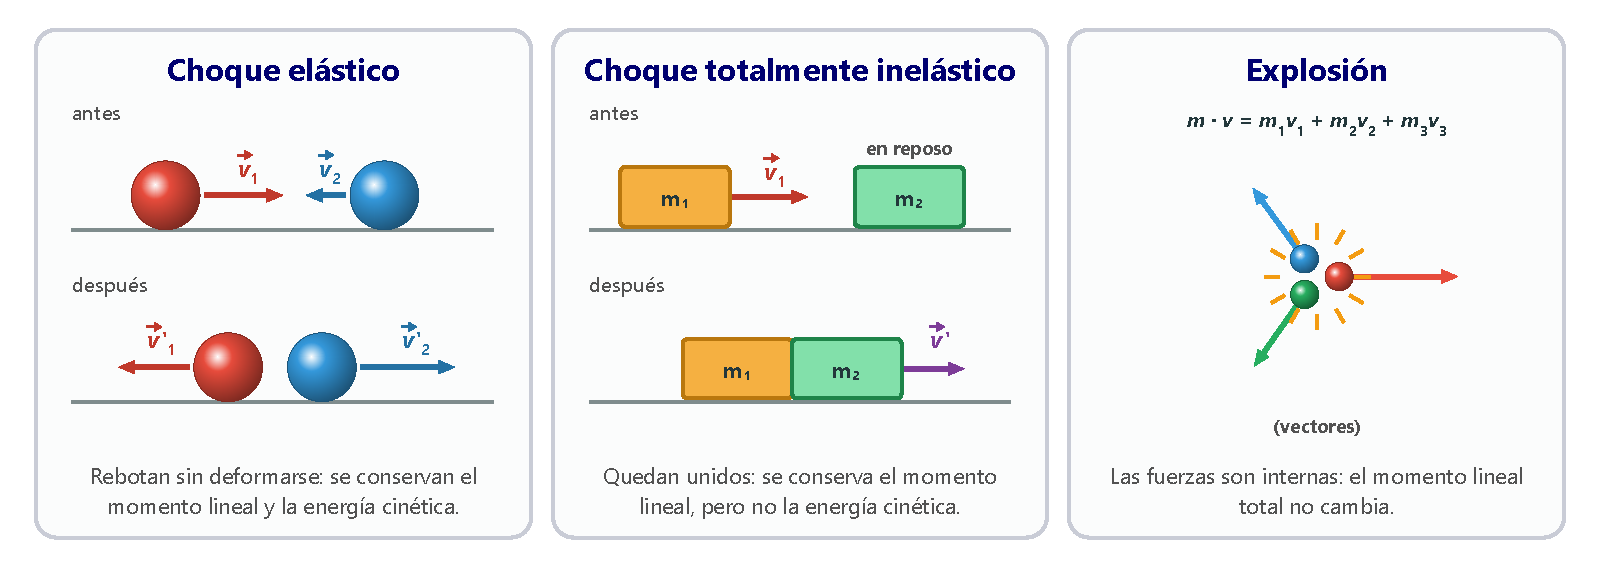
\includegraphics[width=\textwidth]{images/UD10/choques}
    \caption{En choques y explosiones el momento lineal total del sistema se conserva.}
    \label{fig:ud10-choques}
\end{figure}

\begin{example}
    \textbf{Un choque en dos dimensiones.} En una partida de billar, la bola blanca, de \qty{170}{\g}, choca a \qty{3}{\m\per\s} con
    una bola de \qty{160}{\g} en reposo. Tras el choque, esta sale a \qty{2.4}{\m\per\s} formando \(25^\circ\) con la dirección
    inicial de la blanca. ¿Qué velocidad tiene la bola blanca después del choque?

    \textbf{Solución.} Tomamos el eje \(X\) en la dirección inicial de la blanca (A); la otra bola es B.
    \[ \vec{p}_0 = m_A\,\vec{v}_A = \num{0.17} \cdot 3\,\ivec = \num{0.51}\,\ivec~\unit{\kg\m\per\s} \]
    \[ \vec{p}\,'_B = \num{0.16} \cdot (\num{2.4}\cos 25^\circ\,\ivec + \num{2.4}\sen 25^\circ\,\jvec) = (\num{0.348}\,\ivec + \num{0.162}\,\jvec)~\unit{\kg\m\per\s} \]
    Como el momento lineal se conserva, \(\vec{p}_0 = m_A\,\vec{v}\,'_A + \vec{p}\,'_B\):
    \[ \vec{v}\,'_A = \frac{\num{0.51}\,\ivec - (\num{0.348}\,\ivec + \num{0.162}\,\jvec)}{\num{0.17}} = (\num{0.95}\,\ivec - \num{0.95}\,\jvec)~\unit{\m\per\s} \]
    Su módulo es \(\qty{1.35}{\m\per\s}\) y forma \(45^\circ\) por debajo de la dirección inicial.
\end{example}

\begin{exercise}
    Para estudiar el efecto de un disparo, se dispara contra un maniquí de \qty{75}{\kg} en reposo sobre una superficie sin
    rozamiento una bala de \qty{10}{\g}, que se queda incrustada. Si el maniquí adquiere una velocidad de \qty{0.12}{\m\per\s}, ¿cuál
    era la velocidad de la bala?
    \begin{solu}
        \textcolor{blue}{Choque totalmente inelástico: \(m\,v = (m + M)\,v'\).}
        \(v = \dfrac{\num{75.01} \cdot \num{0.12}}{\num{0.010}} = \textcolor{red}{\qty{900}{\m\per\s}}\).
    \end{solu}
\end{exercise}

\begin{exercise}
    Un murciélago de \qty{12}{\g} vuela a \qty{8}{\m\per\s} y caza un insecto de \qty{0.5}{\g} que vuela a \qty{1}{\m\per\s} en la
    misma dirección y sentido. ¿Qué velocidad tiene el murciélago justo después de atraparlo?
    \begin{solu}
        \(v' = \dfrac{\num{0.012} \cdot 8 + \num{0.0005} \cdot 1}{\num{0.0125}} = \textcolor{red}{\qty{7.72}{\m\per\s}}\).
    \end{solu}
\end{exercise}

\begin{exercise}
    En un espectáculo de fuegos artificiales, un cohete de \qty{900}{\g} sube verticalmente y, cuando va a \qty{25}{\m\per\s},
    explota en tres trozos. Un trozo de \qty{300}{\g} sigue subiendo a \qty{40}{\m\per\s}; otro de \qty{250}{\g} sale horizontalmente
    hacia la derecha a \qty{30}{\m\per\s}. Calcula la velocidad del tercer trozo.
    \begin{solu}
        \textcolor{blue}{\(\vec{p} = \num{0.9} \cdot 25\,\jvec = \num{22.5}\,\jvec\); \(\vec{p}_1 = 12\,\jvec\);
        \(\vec{p}_2 = \num{7.5}\,\ivec\); \(\vec{p}_3 = \vec{p} - \vec{p}_1 - \vec{p}_2 = -\num{7.5}\,\ivec + \num{10.5}\,\jvec\).}
        \(\vec{v}_3 = \dfrac{\vec{p}_3}{\num{0.35}} = \textcolor{red}{(-\num{21.4}\,\ivec + 30\,\jvec)~\unit{\m\per\s}}\) (módulo
        \qty{36.9}{\m\per\s}).
    \end{solu}
\end{exercise}

%========================================================================================
\section{El momento angular}\label{sec:ud10-momento-angular}
%========================================================================================

En los apartados anteriores hemos estudiado la \textbf{traslación}: las fuerzas cambian la velocidad de un cuerpo y, sin fuerza
exterior neta, el momento lineal se conserva. Para la \textbf{rotación} hemos visto que el momento de una fuerza puede cambiar la
velocidad angular de un cuerpo. ¿Hay una magnitud que desempeñe en los giros el papel del momento lineal? Sí: el \textbf{momento
angular}.

\subsection{Concepto de momento angular}

\begin{definition}[Momento angular o cinético]
    El momento angular de una partícula respecto a un punto O es el producto vectorial de su vector de posición respecto a O por su
    momento lineal:
    \[ \vec{L} = \vec{r} \times \vec{p} = \vec{r} \times m\,\vec{v} \]
    Su unidad en el SI es el \unit{\kg\m\squared\per\s}.
\end{definition}

No es una propiedad del cuerpo solo: depende del punto O que se elija. Sus características son (figura~\ref{fig:ud10-angular}):
\begin{itemize}
    \item \textbf{Módulo}: \(L = r\,p\sen\alpha = r\,m\,v\sen\alpha\), donde \(\alpha\) es el ángulo entre \(\vec{r}\) y \(\vec{p}\).
    \item \textbf{Dirección}: perpendicular al plano que forman \(\vec{r}\) y \(\vec{p}\).
    \item \textbf{Sentido}: el que da la \textbf{regla de la mano derecha}: si los dedos de la mano derecha giran de \(\vec{r}\) hacia
    \(\vec{p}\) por el camino más corto, el pulgar indica el sentido de \(\vec{L}\). Es también el sentido en que avanza un sacacorchos
    que gira como la partícula.
\end{itemize}
Si \(\vec{r}\) y \(\vec{p}\) tienen la misma dirección (\(\alpha = 0^\circ\) o \(180^\circ\)), el momento angular es nulo. En un
\textbf{movimiento circular} respecto al centro, \(\vec{r}\) y \(\vec{v}\) son siempre perpendiculares y, como \(v = \omega\,r\),
\[ L = m\,v\,r = m\,\omega\,r^2 \]

\begin{figure}[H]
    \centering
    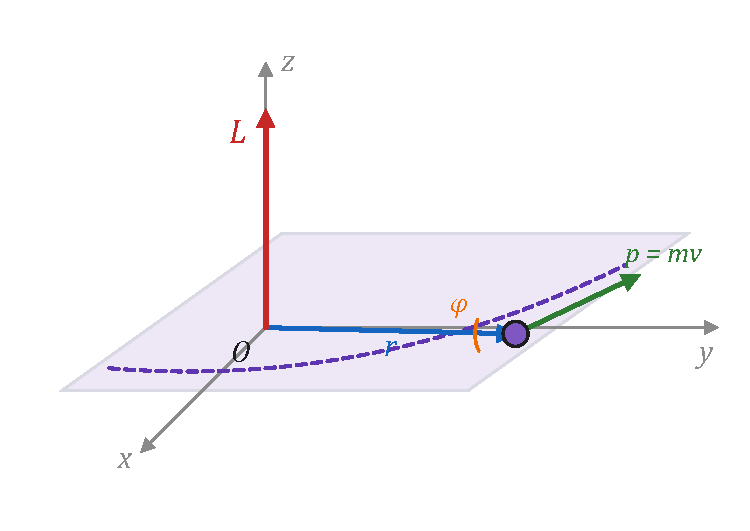
\includegraphics[width=0.55\textwidth]{images/UD10/momento_angular}
    \caption{Momento angular de una partícula respecto a O: perpendicular al plano que forman \(\vec{r}\) y \(\vec{p}\).}
    \label{fig:ud10-angular}
\end{figure}

\begin{example}
    \textbf{En el tiovivo.} Un niño de \qty{25}{\kg} va montado en un tiovivo a \qty{3}{\m} del eje, que gira a \qty{6}{rpm}. Calcula
    su momento angular respecto al eje.

    \textbf{Solución.} \(\omega = 6 \cdot \dfrac{2\pi}{60} = \qty{0.628}{\radian\per\s}\). Como \(\vec{r}\) y \(\vec{v}\) son perpendiculares:
    \[ L = m\,\omega\,r^2 = 25 \cdot \num{0.628} \cdot 3^2 = \qty{141}{\kg\m\squared\per\s} \]
\end{example}

\subsection{Momento de una fuerza y momento angular}

Igual que la fuerza neta cambia el momento lineal, el momento de la fuerza cambia el momento angular. Derivando \(\vec{L}\) con la
regla del producto:
\[ \frac{\dif\vec{L}}{\dif t} = \frac{\dif\vec{r}}{\dif t} \times \vec{p} + \vec{r} \times \frac{\dif\vec{p}}{\dif t}
= \vec{v} \times m\,\vec{v} + \vec{r} \times \vec{F} = \vec{r} \times \vec{F} \]
porque el producto vectorial de dos vectores paralelos es nulo. Por tanto:
\[ \frac{\dif\vec{L}}{\dif t} = \vec{M} \]
Esta es la \textbf{ecuación fundamental de la dinámica de rotación}: la variación del momento angular por unidad de tiempo es igual
al momento de la fuerza neta.

\subsection{Conservación del momento angular}

\begin{definition}[Principio de conservación del momento angular]
    Si el momento resultante de las fuerzas exteriores respecto a un punto O es nulo, el momento angular respecto a ese punto
    permanece constante:
    \[ \vec{M} = \vec{0} = \frac{\dif\vec{L}}{\dif t} \;\Rightarrow\; \vec{L} = \text{constante} \]
\end{definition}

El momento \(\vec{M} = \vec{r} \times \vec{F}\) es nulo en dos casos:
\begin{itemize}
    \item Cuando la fuerza neta es nula.
    \item Cuando \(\vec{r}\) y \(\vec{F}\) son paralelos. Es lo que ocurre con las \textbf{fuerzas centrales}, cuya dirección pasa siempre
    por un punto fijo, como la fuerza de un muelle o la atracción gravitatoria del Sol sobre los planetas.
\end{itemize}

\paragraph{El movimiento de los planetas.} La fuerza con que el Sol atrae a la Tierra es central: está dirigida siempre hacia el Sol
y es paralela al vector de posición. Por eso el momento angular de la Tierra respecto al Sol es constante, y de ahí se deducen dos
cosas: la \textbf{trayectoria es plana} (la dirección de \(\vec{L}\) no cambia) y el planeta va \textbf{más rápido cuanto más cerca
está del Sol} (\(r\,v\) es constante en los puntos en que \(\vec{r}\) y \(\vec{v}\) son perpendiculares). Lo mismo ocurre con todos los
planetas y satélites.

\begin{remark}
    Una patinadora que gira con los brazos extendidos gira mucho más deprisa al recogerlos: al acercar la masa al eje, disminuye
    \(r\) y, para que \(L\) se mantenga, aumenta la velocidad angular.
\end{remark}

\begin{example}
    \textbf{La órbita de la Luna.} En su punto más cercano a la Tierra (perigeo), a \qty{363300}{\km}, la Luna se mueve a
    \qty{3880}{\km\per\hour}; en el más alejado (apogeo), a \qty{3460}{\km\per\hour}. Calcula la distancia Tierra-Luna en el apogeo.

    \textbf{Solución.} La fuerza que la Tierra ejerce sobre la Luna es central, así que el momento angular se conserva. En el perigeo
    y en el apogeo, \(\vec{r}\) y \(\vec{v}\) son perpendiculares (\(\sen\alpha = 1\)):
    \[ L_p = L_a \Rightarrow r_p\,m\,v_p = r_a\,m\,v_a \Rightarrow r_a = \frac{r_p\,v_p}{v_a} = \frac{363300 \cdot 3880}{3460} = \qty{407400}{\km} \]
    No hace falta conocer la masa de la Luna ni pasar las unidades al SI, porque se simplifican.
\end{example}

\begin{exercise}
    Calcula el momento angular del minutero de un reloj de torre respecto al eje. Supón que su masa, \qty{30}{\kg}, está concentrada
    a \qty{1.2}{\m} del eje.
    \begin{solu}
        \(\omega = \dfrac{2\pi}{3600} = \qty{1.745e-3}{\radian\per\s}\); \(L = m\,\omega\,r^2 = 30 \cdot \num{1.745e-3} \cdot \num{1.2}^2 =
        \textcolor{red}{\qty{7.54e-2}{\kg\m\squared\per\s}}\).
    \end{solu}
\end{exercise}

\begin{exercise}
    En el punto de su órbita más cercano al Sol (perihelio), Marte está a \qty{1.38}{UA} y se mueve a \qty{26.5}{\km\per\s}. En el
    más alejado (afelio), está a \qty{1.67}{UA}. ¿Qué velocidad lleva en el afelio?
    \begin{solu}
        \(v_a = \dfrac{r_p\,v_p}{r_a} = \dfrac{\num{1.38} \cdot \num{26.5}}{\num{1.67}} = \textcolor{red}{\qty{21.9}{\km\per\s}}\).
    \end{solu}
\end{exercise}

%========================================================================================
\section{Física en la vida: el bosón de Higgs y el CERN}\label{sec:ud10-higgs}
%========================================================================================

El 4 de julio de 2012, el \textbf{CERN} (Organización Europea para la Investigación Nuclear), en Ginebra, anunció el descubrimiento de
una partícula buscada durante casi medio siglo: el \textbf{bosón de Higgs}. Según el \textbf{Modelo Estándar}, la teoría que describe las
partículas elementales y tres de las cuatro interacciones fundamentales, este bosón está asociado a un campo que llena todo el
espacio y que es el responsable de que las partículas elementales tengan masa.

El hallazgo se hizo en el \textbf{Gran Colisionador de Hadrones} (LHC), un anillo de \qty{27}{\km} de circunferencia situado a unos
\qty{100}{\m} bajo tierra, en la frontera entre Suiza y Francia. En él, dos haces de protones circulan en sentidos opuestos a una
velocidad muy cercana a la de la luz, guiados por imanes superconductores enfriados a \qty{-271.3}{\celsius}, más fríos que el espacio
exterior. Cuando los protones chocan, su enorme energía se convierte en nuevas partículas.

El bosón de Higgs no se observa directamente, porque se desintegra casi al instante. Lo que se detecta son las partículas en que se
desintegra, y para reconstruir lo ocurrido se aplica la \textbf{conservación del momento lineal} (y de la energía) en cada choque. Los
grandes detectores del LHC (ATLAS, CMS, LHCb y ALICE) son, en cierto modo, enormes cámaras que fotografían choques y explosiones de
partículas. El descubrimiento valió el Premio Nobel de Física de 2013 a \textbf{Peter Higgs} y \textbf{François Englert}, que habían
predicho la partícula en 1964.

En el CERN trabajan miles de científicos de todo el mundo. España es estado miembro desde 1983 y cientos de investigadores, ingenieros
y técnicos españoles participan en sus experimentos; entre ellos, la física \textbf{María José Costa}, elegida en 2024 portavoz (máxima
responsable) de la colaboración ATLAS, uno de los dos grandes detectores que descubrieron el Higgs.

\begin{exercise}
    a) En un choque en el LHC, dos protones de igual masa se mueven en la misma dirección y sentidos opuestos con la misma rapidez.
    ¿Cuál es el momento lineal total antes del choque? ¿Qué podemos decir del momento lineal total de todas las partículas que se
    producen? b) Un núcleo en reposo se desintegra en dos fragmentos de masas \(m\) y \(4m\). Si el ligero sale a
    \qty{1.5e7}{\m\per\s}, ¿qué velocidad tiene el pesado? c) Investigad qué otras partículas se han descubierto en aceleradores y
    en qué consisten los cuatro grandes experimentos del LHC.
    \begin{solu}
        a) \(\vec{p} = m\,\vec{v} + m\,(-\vec{v}) = \textcolor{red}{\vec{0}}\); \textcolor{red}{la suma vectorial de los momentos de
        todas las partículas producidas también debe ser nula}. b) \(0 = m \cdot \num{1.5e7} + 4m\,v \Rightarrow
        \textcolor{red}{v = \qty{-3.75e6}{\m\per\s}}\) (en sentido contrario). c) \textcolor{red}{Respuesta abierta} (por ejemplo,
        los bosones W y Z, el quark top, el antiprotón).
    \end{solu}
\end{exercise}

%========================================================================================
\section{Prácticas}\label{sec:ud10-practicas}
%========================================================================================

\subsection{Las tres leyes de la dinámica en casa}

\noindent\begin{minipage}[t]{0.48\textwidth}
    \textbf{Objetivo}
    \begin{itemize}
        \item Comprobar las tres leyes de Newton con materiales caseros.
    \end{itemize}
\end{minipage}\hfill
\begin{minipage}[t]{0.48\textwidth}
    \textbf{Material}
    \begin{itemize}
        \item Un vaso, una cartulina, una moneda, un coche de juguete, una cuerda, unos bloques o piezas de construcción, una pajita, un
        globo y cinta adhesiva.
    \end{itemize}
\end{minipage}

\textbf{Procedimiento}
\begin{enumerate}[label=\numberballgreen]
    \item \textbf{Primera ley.} Tapa el vaso con la cartulina y pon la moneda encima, sobre la boca del vaso. Da un golpe seco y
    horizontal a la cartulina con el dedo: la cartulina sale disparada y la moneda cae dentro del vaso.
    \item \textbf{Segunda ley.} Ata el coche de juguete a una cuerda que pase por el borde de una mesa y cuelga del otro extremo unos
    bloques. Al soltarlos, el peso de los bloques acelera el coche. Repite la experiencia con más bloques colgando y, después,
    cargando el coche con más masa, y observa cómo cambia la aceleración.
    \item \textbf{Tercera ley.} Pasa una cuerda larga por la pajita y átala tensa entre dos puntos de una habitación. Infla el globo
    sin cerrarlo, sujétalo con cinta adhesiva a la pajita y suéltalo: el aire sale hacia atrás y el globo avanza hacia delante por la
    cuerda.
\end{enumerate}

\begin{exercise}
    a) ¿Por qué la moneda no sale despedida junto con la cartulina? ¿Qué ocurre si empujas la cartulina despacio? b) En la segunda
    experiencia, ¿qué ocurre con la aceleración si se duplican los bloques que cuelgan? ¿Y si se duplica la masa del coche?
    c) Identifica la acción y la reacción en el globo. ¿Qué le ocurriría al globo si no estuviera en la cuerda?
    \begin{solu}
        a) \textcolor{red}{Por inercia}: el golpe es tan breve que el rozamiento apenas actúa y la moneda sigue en reposo; al quitar la
        cartulina, cae por su peso. Si se empuja despacio, el rozamiento actúa más tiempo y la moneda se mueve con la cartulina.
        b) \textcolor{red}{Aumenta} (aunque no llega a duplicarse, porque también aumenta la masa total que se acelera);
        \textcolor{red}{disminuye}. c) \textcolor{red}{Acción: el globo empuja el aire hacia atrás; reacción: el aire empuja el globo
        hacia delante.} Sin la cuerda, el globo se movería de forma desordenada porque la dirección del chorro cambia continuamente.
    \end{solu}
\end{exercise}

\subsection{La segunda ley con un carrito}

\noindent\begin{minipage}[t]{0.48\textwidth}
    \textbf{Objetivo}
    \begin{itemize}
        \item Medir la aceleración de un carrito arrastrado por una masa que cuelga y compararla con la que predice la segunda ley.
    \end{itemize}
\end{minipage}\hfill
\begin{minipage}[t]{0.48\textwidth}
    \textbf{Material}
    \begin{itemize}
        \item Un carrito de laboratorio (o un coche de juguete con buenas ruedas), una polea, hilo, pesas, una balanza, una cinta
        métrica y un cronómetro (o el móvil para grabar en vídeo).
    \end{itemize}
\end{minipage}

\begin{figure}[H]
    \centering
    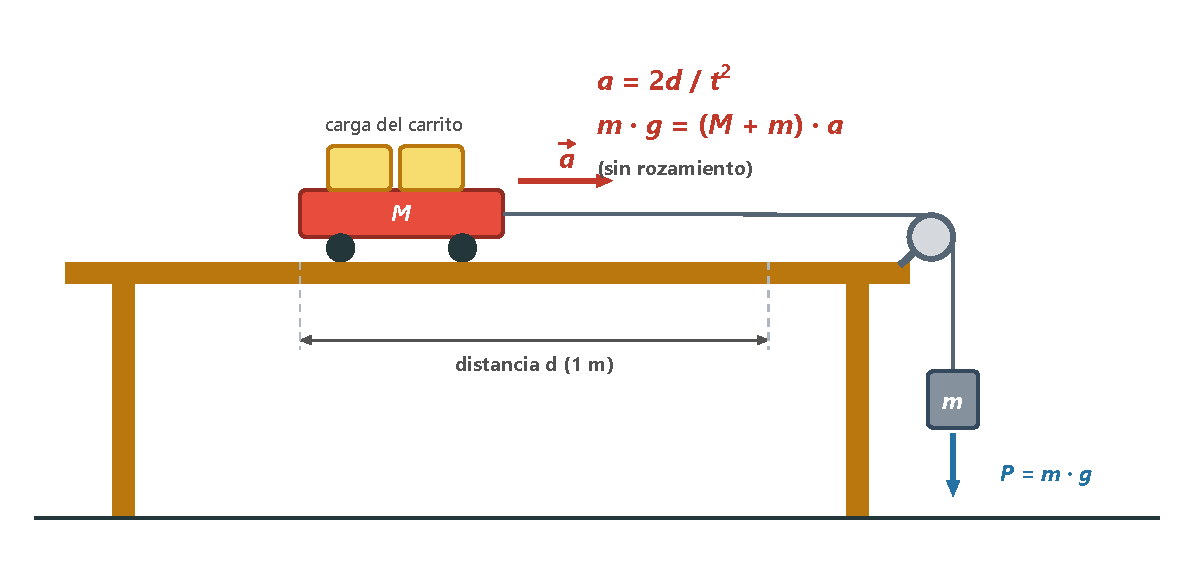
\includegraphics[width=0.75\textwidth]{images/UD10/practica_carrito}
    \caption{El peso de la masa que cuelga acelera todo el sistema: el carrito y la propia masa.}
    \label{fig:ud10-carrito}
\end{figure}

\textbf{Procedimiento}
\begin{enumerate}[label=\numberballgreen]
    \item Mide con la balanza la masa \(M\) del carrito y la masa \(m\) que vas a colgar.
    \item Monta el dispositivo de la figura~\ref{fig:ud10-carrito} y marca en la mesa una distancia \(d = \qty{1}{\m}\).
    \item Suelta el carrito desde el reposo y mide el tiempo \(t\) que tarda en recorrer esa distancia. Repite la medida tres veces y
    calcula el tiempo medio. La aceleración es \(a = 2d/t^2\).
    \item Cambia la masa que cuelga (y luego la carga del carrito) y anota los resultados en una tabla.
\end{enumerate}

\begin{exercise}
    a) Demuestra que, sin rozamiento, la aceleración del sistema es \(a = \dfrac{m\,g}{M + m}\). b) Con \(M = \qty{450}{\g}\) y
    \(m = \qty{50}{\g}\), un grupo mide un tiempo medio de \qty{1.50}{\s} para recorrer \qty{1}{\m}. Calcula la aceleración medida
    y la teórica. c) ¿A qué puede deberse la diferencia? Calcula la fuerza de rozamiento que la explicaría.
    \begin{solu}
        a) \textcolor{blue}{Sobre el sistema (carrito y pesa), la fuerza neta es el peso de la pesa, y la masa que se acelera es la
        total:} \(\textcolor{red}{m\,g = (M + m)\,a}\). b) Medida: \(a = \dfrac{2 \cdot 1}{\num{1.50}^2} =
        \textcolor{red}{\qty{0.89}{\m\per\s\squared}}\); teórica: \(a = \dfrac{\num{0.05} \cdot \num{9.8}}{\num{0.5}} =
        \textcolor{red}{\qty{0.98}{\m\per\s\squared}}\). c) Al \textcolor{red}{rozamiento} (y a los errores al cronometrar):
        \(F_r = m\,g - (M + m)\,a = \num{0.49} - \num{0.5} \cdot \num{0.889} = \textcolor{red}{\qty{0.046}{\newton}}\).
    \end{solu}
\end{exercise}

%========================================================================================
\section{Situación de aprendizaje: cohetes espaciales y cohetes de agua (ODS 9)}\label{sec:ud10-cohetes}
%========================================================================================

Un cohete es un vehículo diseñado para llevar cargas útiles, como satélites, sondas o personas, de la Tierra al espacio. Su
funcionamiento se basa en la \textbf{tercera ley de Newton}: los motores queman una gran cantidad de combustible y expulsan los gases a
gran velocidad hacia abajo; los gases, a su vez, empujan al cohete hacia arriba. Visto de otro modo, es la \textbf{conservación del
momento lineal}: el momento que ganan los gases hacia abajo lo gana el cohete hacia arriba. Los cohetes reutilizables, que aterrizan
para volver a usarse, son un buen ejemplo de la innovación que promueve el \textbf{ODS 9} (industria, innovación e infraestructura).

\begin{marker}
    \textbf{Reto:} por grupos, investigad sobre los cohetes y construid un \textbf{cohete de agua} con materiales reciclados. Grabad un
    vídeo del lanzamiento y preparad un informe que explique su funcionamiento con las leyes de la dinámica.
\end{marker}

\begin{enumerate}[label=\numberballred]
    \item \textbf{Investigad sobre Newton}: su biografía, los científicos que lo inspiraron, sus experimentos y cómo formuló las leyes
    de la dinámica.
    \item \textbf{Investigad sobre los cohetes}: historia y científicos destacados, partes de un cohete, cómo funcionan y cohetes
    actuales y futuros.
    \item \textbf{Relacionad los cohetes con la dinámica}: el empuje y el peso, la velocidad de salida de los gases, la masa del cohete
    y de la carga útil, la velocidad de escape. ¿El empuje tiene que ser mayor que el peso?
    \item \textbf{Construid el cohete de agua} con una botella de plástico, aletas de cartón, agua y una bomba de bicicleta con un tapón
    adaptado. Diseñad la plataforma de lanzamiento, haced un presupuesto y lanzadlo en un lugar despejado y con supervisión.
\end{enumerate}

\begin{exercise}
    a) Un cohete de \qty{2.6e6}{\kg} produce al despegar un empuje de \qty{39}{\mega\newton}. Calcula su aceleración inicial. ¿Qué
    ocurriría si el empuje fuera menor que su peso? b) Un cohete expulsa cada segundo \qty{1200}{\kg} de gases a \qty{3000}{\m\per\s}.
    Calcula el empuje con el teorema del impulso. c) En un cohete de agua de \qty{0.3}{\kg} (vacío), sale \qty{0.5}{\kg} de agua a
    \qty{15}{\m\per\s} en muy poco tiempo. Estima la velocidad que adquiere el cohete (sin tener en cuenta el peso ni el aire).
    \begin{solu}
        a) \(a = \dfrac{F - m\,g}{m} = \dfrac{\num{39e6}}{\num{2.6e6}} - \num{9.8} = \textcolor{red}{\qty{5.2}{\m\per\s\squared}}\).
        \textcolor{red}{Si el empuje fuera menor que el peso, el cohete no despegaría.} b) \(F = \dfrac{\Delta p}{\Delta t} =
        \dfrac{1200 \cdot 3000}{1} = \textcolor{red}{\qty{3.6e6}{\newton}}\). c) Conservación del momento lineal:
        \(\num{0.3}\,v = \num{0.5} \cdot 15 \Rightarrow \textcolor{red}{v = \qty{25}{\m\per\s}}\) (el valor real es menor, porque el
        agua sale poco a poco y actúan el peso y el rozamiento con el aire).
    \end{solu}
\end{exercise}
